%%
%% Copyright 2019-2020 Elsevier Ltd
%%
%% This file is part of the 'CAS Bundle'.
%%
%% Template article for cas-dc documentclass (double column output).
%% Paper: CSAR-Net for long-tailed magnetic tile surface defect recognition.
%%
%% Module-stitching narrative: each of the three modules (backbone -> CBAM
%% attention -> LDAM loss) is introduced in sequence, and their decoupled
%% collaboration (plus the collapsed CS-CBAM counter-design) is made explicit.

\documentclass[a4paper,fleqn]{cas-sc}

\usepackage[authoryear]{natbib}
\usepackage{hyperref}
\usepackage{graphicx}
\usepackage{subfigure}
\usepackage{epstopdf}
\usepackage{color}
\usepackage{booktabs}
\usepackage{amsmath}
\usepackage{multirow}
\usepackage{tikz}
\usetikzlibrary{positioning,arrows.meta,fit,calc,shadows}

%%% Author definitions
\def\tsc#1{\csdef{#1}{\textsc{\lowercase{#1}}\xspace}}
\tsc{WGM}
\tsc{QE}
\tsc{EP}
\tsc{PMS}
\tsc{BEC}
\tsc{DE}
%%%

\begin{document}
\begin{sloppypar}
	\let\WriteBookmarks\relax
	\def\floatpagefraction{0.7}
	\def\textfraction{0.05}
	\def\topfraction{0.85}
	\def\bottomfraction{0.85}
	\let\printorcid\relax
	\shorttitle{CSAR-Net for Long-Tailed Magnetic Tile Defect Recognition}
	\shortauthors{C. Xie et~al.}

	%% Title
	\title [mode = title]{CSAR-Net: A Cost-Sensitive Attention Residual Network for Long-Tailed Magnetic Tile Surface Defect Recognition}

	%% Authors
	\author[1]{[First author]}
	\cormark[1]
	\ead{[Corresponding email]}

	\author[1]{Chenyang Xie}
	\ead{[Second author email]}

	\address[1]{[Affiliation], China}

	\cortext[cor1]{Corresponding author.}

	%% Abstract
	\begin{abstract}
		Magnetic tiles are the core magnetic components of permanent-magnet motors and related equipment, and surface defect inspection is a decisive step in their manufacturing quality control. Real production lines exhibit a naturally long-tailed defect distribution, in which defect-free samples dominate while break and fray defects are scarce; the economic cost of missing such defects far exceeds that of false alarms. Existing convolutional neural network (CNN) methods mostly optimize average accuracy and thereby ignore both the long-tailed distribution and the asymmetry of miss costs. To remedy this, we propose a Cost-Sensitive Attention Residual Network, CSAR-Net, assembled from three decoupled modules: (i) a ResNet18 backbone for hierarchical feature extraction; (ii) the Convolutional Block Attention Module (CBAM) inserted into the residual blocks of stages 3 and 4 for label-agnostic feature refinement; and (iii) the Label-Distribution-Aware Margin (LDAM) loss applied in the loss layer for label-dependent cost-sensitive calibration. The name follows the convention of combining the initials of the innovation and the base architecture. Multi-seed (3 seeds) experiments on the real Magnetic Tile Surface Defects (MTSD) dataset (6 classes, natural imbalance $\approx$ 30:1) show that feature-layer attention is the robust source of improvement: CBAM alone raises macro G-mean from 0.752 to 0.782 ($+$3.1pp) with the lowest variance across all configurations, and lifts the recall of the hardest, costliest break defect from 0.490 to 0.549 while keeping defect-free recall nearly intact. A systematic ablation covering module contributions, injection position, channel/spatial decomposition, and margin-coefficient sensitivity shows that every form of loss-layer cost calibration over-corrects on this small real dataset (the full LDAM loss by $-$8.6pp, its margin-only and reweighting-only variants by $-$3.8pp and $-$4.8pp), and that stacking LDAM on top of CBAM dilutes the attention gain from 0.782 to 0.744. Injecting the cost signal directly into attention (the coupled CS-CBAM variant) collapses to the majority class because of train/inference inconsistency. These results answer a central design question: the cost-sensitive signal should act in the feature layer through label-agnostic attention rather than in the loss layer through reweighting. We further derive managerial implications for inspection systems from quality-cost theory.
	\end{abstract}

	%% Highlights
	\begin{highlights}
		\item A Cost-Sensitive Attention Residual Network (CSAR-Net) is proposed for magnetic tile defect recognition.
		\item Three modules(backbone, CBAM attention, and LDAM loss)are decoupled and combined.
		\item Feature-layer CBAM attention is the robust gain: $+$3.1pp macro G-mean with the lowest variance, lifting break-defect recall from 0.490 to 0.549 on MTSD.
		\item Loss-layer cost calibration over-corrects in every form ($-$3.8pp to $-$8.6pp), and stacking it on CBAM dilutes the gain.
		\item Injecting the cost signal into attention (CS-CBAM) collapses due to train/inference inconsistency.
	\end{highlights}

	%% Keywords
	\begin{keywords}
		Surface defect detection \sep
		Magnetic tile \sep
		Convolutional neural network \sep
		Attention mechanism \sep
		Long-tailed recognition \sep
		Cost-sensitive learning
	\end{keywords}

	\maketitle

	%% 1. Introduction
	\section{Introduction}
	\label{sec:intro}

	\par{
		Magnetic tiles are the core magnetic components of permanent-magnet motors, loudspeakers, and sensors, and their surface defects (blowhole, break, crack, fray, and unevenness) directly determine product performance and safety \citep{huang2020surface}. Traditional manual inspection is subjective, lagging, and difficult to scale, and statistical process control \citep{montgomery2013introduction} alone cannot guarantee zero defects for safety-critical components. Automated defect recognition based on convolutional neural networks (CNNs) has therefore become a key enabling technology in intelligent manufacturing \citep{xie2021ffcnn,chen2021surface}. Over the past few years, researchers have proposed a succession of deep-learning solutions for magnetic tile defects, such as the fusion feature CNN (FFCNN) \citep{xie2021ffcnn}, the convolutional retinal attention block (CRAB) \citep{li2024attention}, and the lightweight parallel attention residual network (LPAR-Net) \citep{lv2024lightweight}, all reporting high accuracy.
	}

	\par{
		However, most existing methods optimize \emph{average accuracy} and overlook two constraints that hold in real production. One is that defects are naturally long-tailed: defect-free samples dominate while break and fray are scarce. In the MTSD dataset \citep{huang2020surface} used here, there are 952 defect-free images but only 32 of the rarest fray class, an imbalance ratio of about 30:1 (Fig.~\ref{fig:longtail}). Under such a distribution, a Softmax classifier trained with standard cross-entropy shifts the decision boundary toward the majority class and sharply degrades minority-class recall; in our experiments the cross-entropy baseline reaches a macro G-mean of only 0.752 even though its average accuracy is as high as 0.905. The other constraint is that miss costs are asymmetric: a false alarm (a normal tile judged defective) costs one extra re-inspection, whereas a miss (a defective tile judged normal) lets defective product flow downstream and into the market. Under quality-cost theory the latter belongs to the costliest category, ``external failure cost'' \citep{juran1993quality}. These two constraints mean that neither the training objective nor the evaluation metric may look only at average accuracy; both must explicitly protect the rare, high-cost classes.
	}

	\par{
		Given these constraints, a central and still open question is \emph{at which layer of the network the cost-sensitive signal should act}, the feature-layer attention weights or the loss-layer calibration. We address it by proposing a Cost-Sensitive Attention Residual Network, CSAR-Net, which assembles three modules that are \emph{decoupled} by design. CBAM \citep{woo2018cbam} refines discriminative features in the feature layer, LDAM \citep{cao2019learning} performs cost-sensitive margin and reweighting calibration in the loss layer, and a ResNet18 backbone \citep{he2016deep} supplies the hierarchical representation. We further implement the intermediate variants and the ``coupled'' counter-design CS-CBAM, so that each module's contribution and the correct placement of the cost signal can be isolated.
	}

	\par{
		To make the investigation concrete and auditable, we decompose the central design question into three research questions (RQs). RQ1 (\emph{which module helps?}) asks whether feature-layer attention or loss-layer cost calibration improves long-tailed defect recognition, and by how much. RQ2 (\emph{where should the cost signal act?}) asks whether the label-dependent cost signal is better realized in the feature path, in the training objective, or at the decision rule. RQ3 (\emph{do the modules compose?}) asks whether the attention and cost-calibration modules combine additively, or whether one dilutes the other. Each question is answered by a dedicated, controlled experiment in Section \ref{sec:exp}, so that the conclusion about the correct placement of the cost signal follows from evidence rather than from a single headline number.
	}

	\par{
		Multi-seed experiments on MTSD yield three clear findings. First, feature-layer attention is the robust source of gain: CBAM alone raises macro G-mean by $+$3.1pp and attains the lowest variance among all configurations. Second, loss-layer cost calibration over-corrects in every form: full LDAM loses 8.6pp, while its margin-only and reweighting-only variants lose 3.8pp and 4.8pp. Third, the two modules do not combine additively; stacking LDAM on top of CBAM reduces the attention gain to $-$0.8pp, and injecting the cost signal directly into attention (CS-CBAM) collapses to the majority class owing to train/inference inconsistency. These results localize the correct placement of the cost-sensitive signal to the feature layer, and yield a practical design rule for long-tailed inspection systems.
	}

	\begin{figure}[pos=htbp]
		\centering
		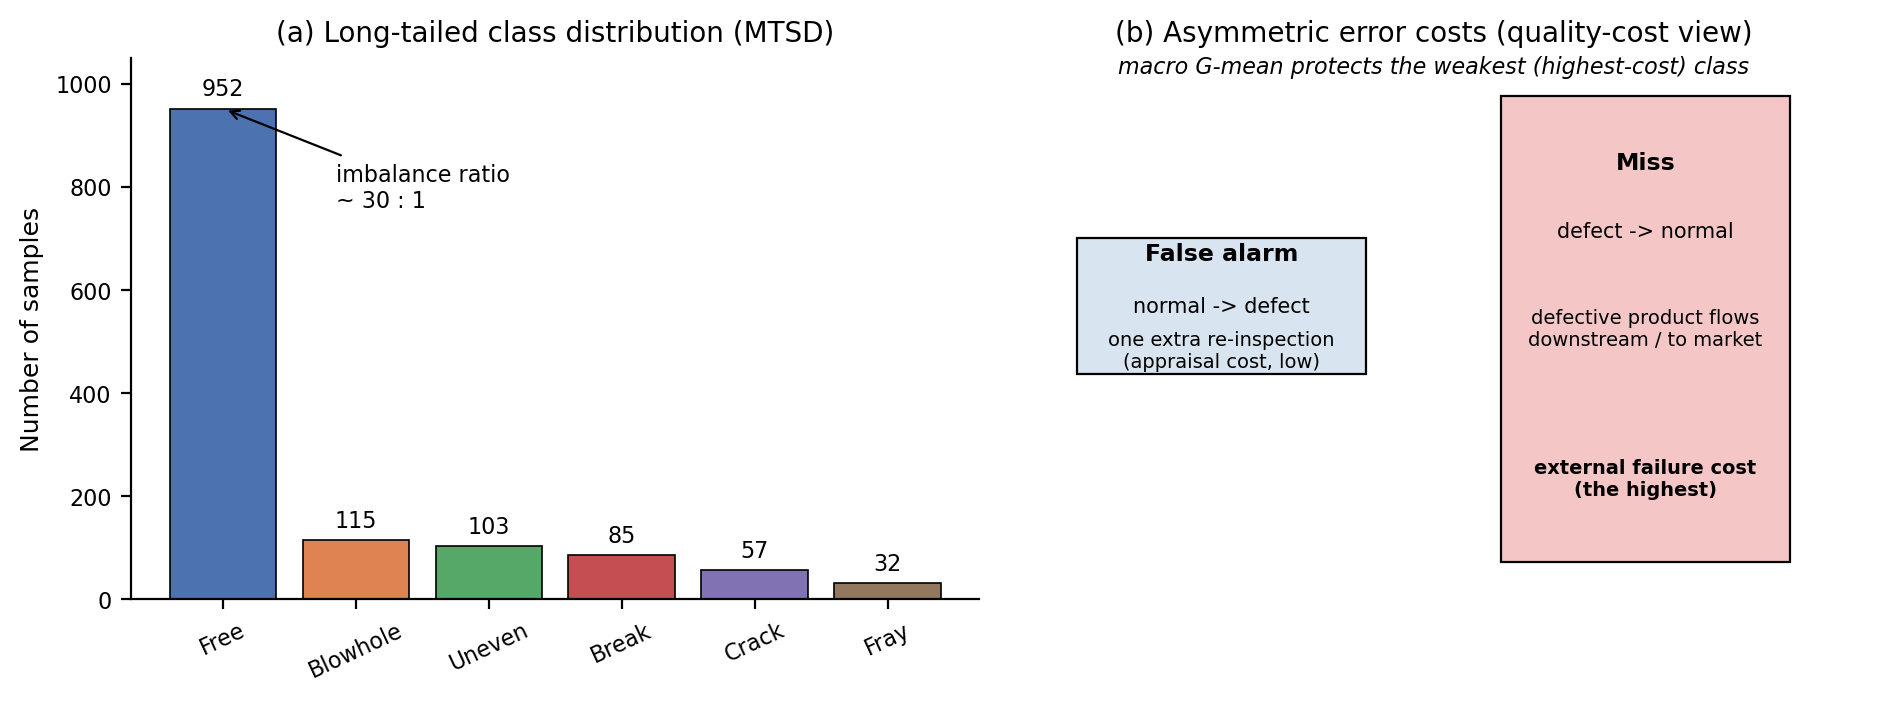
\includegraphics[width=0.95\textwidth]{./figures/longtail_cost.png}
		\caption{The two constraints of real magnetic-tile inspection that motivate CSAR-Net. (a) The long-tailed class distribution of MTSD: defect-free samples dominate while fray is the rarest class (imbalance $\approx$ 30:1). (b) The asymmetry of error costs under quality-cost theory: a false alarm only triggers one re-inspection (appraisal cost), whereas a miss lets defective product flow downstream (external failure cost, the highest). Macro G-mean is the metric that protects the weakest, highest-cost class.}
		\label{fig:longtail}
	\end{figure}

	\par{
		The main contributions of this paper are summarized as follows.
	}

	\begin{enumerate}[(1)]
		\item We propose \textbf{CSAR-Net}, a decoupled three-module framework that combines a ResNet18 backbone, CBAM feature-layer attention, and LDAM loss-layer calibration, and use it to answer \emph{where the cost-sensitive signal should act}: feature-layer attention is the robust source of gain, raising macro G-mean by $+$3.1pp (0.752 to 0.782, the lowest variance) and lifting the hardest break defect from 0.490 to 0.549.
		\item We present a \emph{module-stitching view} of the method: each module is characterized by its input, output, and the property that decides where it belongs in the pipeline (label-agnostic feature refinement vs.\ label-dependent cost calibration), which makes the design transparent and reproducible.
		\item We conduct a \emph{complete ablation}, decomposing the LDAM loss into its margin and reweighting components, sweeping the CBAM injection position and its channel/spatial sub-modules, and testing margin-coefficient sensitivity, thereby localizing both the source of the gain and the cause of the degradation.
		\item We provide a \emph{quality-cost-oriented evaluation}: macro G-mean is adopted as the primary metric to align with the asymmetry of miss and false-alarm costs, and actionable engineering implications are derived from quality-cost theory.
	\end{enumerate}

	\par{
		The rest of this paper is organized as follows. Section \ref{sec:related} reviews related work. Section \ref{sec:method} describes the three modules of CSAR-Net in sequence and how they are stitched together. Section \ref{sec:exp} reports the experimental setup and results, including the ablation. Section \ref{sec:discussion} interprets the mechanism. Section \ref{sec:app} translates the findings into applications and management guidance. Section \ref{sec:conclusion} concludes the paper.
	}

	%% 2. Related work
	\section{Related work}
	\label{sec:related}

	\subsection{Magnetic tile surface defect detection}
	\par{
		Magnetic tile defect detection has evolved from hand-crafted features with shallow classifiers to deep convolutional networks \citep{chen2021surface}. Huang et al.\ \citep{huang2020surface} proposed saliency detection and segmentation for magnetic tile surface defects and released the MTSD dataset, which has since become the standard benchmark for this task. Xie et al.\ \citep{xie2021ffcnn} introduced the fusion feature CNN (FFCNN), which handles multi-view inputs through feature extraction, feature fusion, and decision modules and adds an attention mechanism to focus on representative regions. Li et al.\ \citep{li2024attention} developed the convolutional retinal attention block (CRAB), reporting 99.50\% classification accuracy. Lv et al.\ \citep{lv2024lightweight} presented the lightweight parallel attention residual network (LPAR-Net) with an improved CBAM and inverted bottleneck blocks, reaching 93.63\% accuracy. Beyond classification, Jiang et al.\ \citep{jiang2024mtu2net} designed MT-U2Net for defect localization, Niu et al.\ \citep{niu2025yolordm} proposed YOLO-RDM for efficient defect detection, and Lu et al.\ \citep{lu2022multimodal} combined multimodal fusion with cross-attention for internal defect detection. General-purpose architectures are also widely reused: one-stage detectors such as YOLO \citep{redmon2016you} and segmentation networks such as U-Net \citep{ronneberger2015u} serve defect localization, while classic backbones such as VGG \citep{simonyan2015very} and lightweight variants such as MobileNets \citep{howard2017mobilenets} and MobileNetV2 \citep{sandler2018mobilenetv2} serve deployment-oriented classification. As summarized in Table \ref{tbl:lit}, these works mostly improve accuracy on the same task and rarely address the long-tailed distribution and cost asymmetry of real production, which is the gap this paper targets.
	}

	\subsection{Attention mechanisms}
	\par{
		Attention mechanisms, popularized by the Vision Transformer \citep{dosovitskiy2021image} and subsequently condensed into plug-in CNN modules, improve a network's discriminative ability by adaptively recalibrating feature maps. Squeeze-and-Excitation (SE) \citep{hu2018squeeze} introduces channel attention; the Convolutional Block Attention Module (CBAM) \citep{woo2018cbam} combines channel and spatial attention in series, offering a lightweight and general feature-enhancement means; ECA-Net \citep{wang2020eca} realizes efficient channel attention with one-dimensional convolution; and Coordinate Attention (CA) \citep{hou2021coordinate} embeds positional information into channel attention. For this paper the relevant property is that these operators are \emph{label-agnostic}: they recalibrate features without knowing the class label, and hence behave identically during training and inference. How such an operator interacts with long-tailed cost sensitivity (in particular whether a label-dependent cost signal can be injected into one) has not been studied systematically, and Sections \ref{sec:exp} and \ref{sec:discussion} provide experimental answers. Table \ref{tbl:attnlit} summarizes the four modules compared in Section \ref{sec:attn}; all of them are label-agnostic, but they differ in whether they recalibrate channels only or channels and space jointly, a difference that matters on complex defect textures.
	}

	\begin{table}[pos=htbp]
		\footnotesize
		\caption{Attention modules compared in Section \ref{sec:attn}. All are label-agnostic; the key difference is whether they recalibrate channels only or channels and spatial locations jointly.}
		\label{tbl:attnlit}
		\centering
		\begin{tabular}{llll}
			\hline
			\textbf{Module} & \textbf{Recalibration} & \textbf{Core mechanism} & \textbf{Label-agnostic} \\ \hline
			SE \citep{hu2018squeeze} & channel & GAP $\to$ MLP $\to$ sigmoid gating & Yes \\
			CBAM \citep{woo2018cbam} & channel $+$ spatial (series) & pooled MLP $+$ $7{\times}7$ conv & Yes \\
			ECA \citep{wang2020eca} & channel & $1$D conv (kernel $k$) & Yes \\
			CA \citep{hou2021coordinate} & channel $+$ coordinate & 2D pooling along $h$/$w$ & Yes \\ \hline
		\end{tabular}
	\end{table}

	\subsection{Long-tailed recognition and cost-sensitive learning}
	\par{
		Approaches to class imbalance fall into four families \citep{zhang2023deep}. \emph{Reweighting} scales the per-sample loss by a class-dependent factor: inverse-frequency weighting, the class-balanced loss based on the effective number of samples \citep{cui2019class}, and Focal Loss \citep{lin2017focal}, which down-weights easy samples. \emph{Resampling} balances the training distribution by over-sampling the minority class (e.g., SMOTE \citep{chawla2002smote}) or under-sampling the majority \citep{drummond2003c4}. \emph{Margin losses} enlarge the decision boundary of minority classes, of which LDAM \citep{cao2019learning} (a margin $\Delta_c=C/n_c^{1/4}$ that decays with sample count) is representative. \emph{Decoupling and ensemble methods} separate representation learning from classifier learning \citep{kang2020decoupling}, localizing the long-tail problem to the classifier. A recent review of imbalanced-sample surface defect detection \citep{bai2025surface} summarizes resampling, reweighting, and cost-sensitive methods for defect detection specifically. This paper places attention enhancement and cost-sensitive calibration in a single framework on real magnetic tile data and \emph{decouples} them by layer so that their collaboration can be examined.
	}

	\subsection{Cost-sensitive learning and the decision-rule view}
	\par{
		Cost-sensitive learning extends imbalance handling by assigning explicit misclassification costs rather than only inverse-frequency weights \citep{elkan2001cost,he2009learning}. It admits three distinct insertion points. \emph{(i) The training objective}: cost-matrix reweighting or margin terms, e.g., LDAM \citep{cao2019learning} and Focal Loss \citep{lin2017focal}. \emph{(ii) The feature representation}: cost-aware sampling or synthesis, e.g., SMOTE \citep{chawla2002smote}, or attention. \emph{(iii) The decision rule}: thresholding or re-mapping posterior probabilities against a cost matrix \citep{provost1998cost,elkan2001cost}. An established and often overlooked result is that, for many base learners, moving cost sensitivity from the objective to the decision rule is simpler and more robust \citep{drummond2003c4,elkan2001cost}: reweighting the objective can be unstable on scarce data, whereas a threshold adjustment is reversible and requires no retraining. This three-way distinction organizes our design space: the CSAR-Net ablation compares a feature-layer intervention (CBAM), a loss-layer intervention (LDAM), and a decision-rule intervention (thresholding against $C_{\text{miss}}/C_{\text{re}}$), and finds the feature layer to be the robust choice on this real dataset.
	}

	\subsection{Research gap and positioning}
	\par{
		Table \ref{tbl:lit} condenses the landscape: prior magnetic-tile methods optimize average accuracy and ignore both the long tail and the cost asymmetry, while prior long-tail and cost-sensitive methods are mostly validated on natural-image benchmarks or synthetic data rather than on real industrial surfaces with scarce, visually confusable defects. Three gaps follow. \emph{G1 (evaluation)}: no magnetic-tile method is evaluated under the macro G-mean / miss-cost view, so its behavior on the rarest, costliest defects is unknown. \emph{G2 (interaction)}: whether a label-agnostic attention module and a label-dependent cost signal cooperate or interfere, and whether the cost signal may be injected into attention, lacks a systematic, controlled answer. \emph{G3 (placement)}: the correct \emph{layer} for the cost-sensitive signal (feature, loss, or decision) is rarely treated as a first-class experimental variable. CSAR-Net is designed to close G1--G3: it is evaluated under the miss-cost view on MTSD, it ablates attention/cost interaction with a decoupled vs.\ coupled design, and it varies the placement of the cost signal as an explicit factor.
	}

	\begin{table}[pos=htbp]
		\footnotesize
		\caption{Representative magnetic-tile defect methods. Most optimize average accuracy; few address the long-tailed distribution or the miss/false-alarm cost asymmetry that motivate CSAR-Net.}
		\label{tbl:lit}
		\centering
		\resizebox{\textwidth}{!}{%
			\begin{tabular}{llllcc}
			\hline
			\textbf{Method} & \textbf{Year} & \textbf{Core idea} & \textbf{Reported metric} & \textbf{Long-tail-aware} & \textbf{Cost-aware} \\ \hline
			FFCNN \citep{xie2021ffcnn} & 2021 & Fusion feature CNN $+$ attention & accuracy & No & No \\
			CRAB \citep{li2024attention} & 2024 & Retinal attention block & 99.50\% accuracy & No & No \\
			LPAR-Net \citep{lv2024lightweight} & 2024 & Parallel attention $+$ inverted bottleneck & 93.63\% accuracy & No & No \\
			MT-U2Net \citep{jiang2024mtu2net} & 2024 & Lightweight localization network & localization metrics & No & No \\
			YOLO-RDM \citep{niu2025yolordm} & 2025 & Efficient detection & mAP & No & No \\
			\textbf{CSAR-Net (ours)} & --- & CBAM $+$ LDAM, decoupled & macro G-mean & \textbf{Yes} & \textbf{Yes} \\ \hline
		\end{tabular}}
	\end{table}

	%% 3. Methodology
	\section{Methodology}
	\label{sec:method}

	\par{
		Following the naming convention of convolutional networks, which combine the initials of the innovation and the base architecture (Residual$\rightarrow$ResNet \citep{he2016deep}, Dense$\rightarrow$DenseNet \citep{huang2017densely}), we name the proposed network \textbf{CSAR-Net}, i.e., \textbf{C}ost-\textbf{S}ensitive \textbf{A}ttention \textbf{R}esidual Network, where ``Cost-Sensitive Attention'' is the innovation and ``Residual'' is the base architecture. This section adopts a module-stitching exposition: we first formalize the problem, then introduce the three modules in sequence (the backbone, Module 1; the attention refinement, Module 2; and the cost-sensitive objective, Module 3), and finally describe how they are decoupled and stitched together, together with a coupled counter-design that we show to fail.
	}

	\subsection{Problem formulation}
	\label{sec:problem}
	\par{
		Magnetic tile surface defect recognition is an image classification problem. Given a magnetic tile surface image $\mathbf{x}\in\mathbb{R}^{H\times W\times C}$ (resized to $224\times224\times3$ here, with grayscale replicated into three channels), the task is to predict its defect class among $K=6$ classes $\mathcal{C}=\{\text{blowhole, break, crack, fray, free, uneven}\}$. Let $n_c$ denote the number of training samples of class $c$, and $N=\sum_c n_c$ the total. The dataset is long-tailed: $n_{\text{free}}\gg n_{\text{fray}}$. A model is a function $f_\theta(\mathbf{x})=\text{softmax}(g_\theta(\mathbf{x}))$ mapping an image to a class distribution, where $g_\theta$ is the logit network. The evaluation target is the \emph{macro G-mean}
		\begin{equation}
			\text{G-mean}=\Bigl(\prod_{c=1}^{K}\mathrm{Recall}_c\Bigr)^{1/K},\qquad
			\mathrm{Recall}_c=\frac{TP_c}{TP_c+FN_c},
			\label{eq:gmean}
		\end{equation}
		which, unlike average accuracy, penalizes the weakest class and therefore aligns with the goal of protecting rare defects.
	}

	\begin{table}[pos=htbp]
		\footnotesize
		\caption{Notation used throughout the paper.}
		\label{tbl:notation}
		\centering
		\setlength{\tabcolsep}{2pt}
		\begin{tabular}{ll}
			\hline
			\textbf{Notation} & \textbf{Meaning} \\ \hline
			$\mathbf{x}$, $H{\times}W{\times}C$ & input image (resized to $224{\times}224{\times}3$) \\
			$K$, $\mathcal{C}$ & number of classes ($K=6$) and class set \\
			$n_c$, $N$ & training samples of class $c$ and total ($N=\sum_c n_c$) \\
			$f_\theta$, $g_\theta$ & classifier $f_\theta=\mathrm{softmax}(g_\theta)$ and logit network \\
			$\mathbf{F},\hat{\mathbf{F}},\tilde{\mathbf{F}}$ & raw, channel-refined, and spatial-refined feature map \\
			$M_c$, $M_s$ & channel and spatial attention maps \\
			$\Delta_c$, $C$ & LDAM per-class margin and margin coefficient \\
			$w_c$, $\beta$ & class-balanced weight and effective-number parameter \\
			$\mathrm{Recall}_c$ & per-class recall (Eq.~\eqref{eq:gmean}) \\
			$\pi_c$, $C_{\mathrm{miss}}^{(c)}$ & class prior, per-class miss cost \\
			$C_{\mathrm{re}}$ & re-inspection cost \\ \hline
		\end{tabular}
	\end{table}

	\subsection{Overview of CSAR-Net}
	\label{sec:overview}
	\par{
		Fig.~\ref{fig:arch} shows the overall framework of CSAR-Net. It consists of three modules assembled in a pipeline. \emph{Module 1} is a ResNet18 backbone \citep{he2016deep} with four residual stages (channel counts 64/128/256/512), which extracts a hierarchical feature representation. \emph{Module 2} is a CBAM attention block \citep{woo2018cbam} injected into the residual blocks of stages 3 and 4, which refines the features in a label-agnostic manner. \emph{Module 3} is the LDAM loss \citep{cao2019learning} applied after the classifier, which performs label-dependent cost-sensitive calibration that exists only during training. The 512-dimensional feature after global average pooling is fed into a fully connected classifier that produces six logits. The three modules are \emph{decoupled by layer}: Module 2 operates on features and behaves identically in training and inference, while Module 3 operates on the training objective and vanishes at inference.
	}

	\begin{figure}[pos=htbp]
		\centering
		\resizebox{\textwidth}{!}{%
		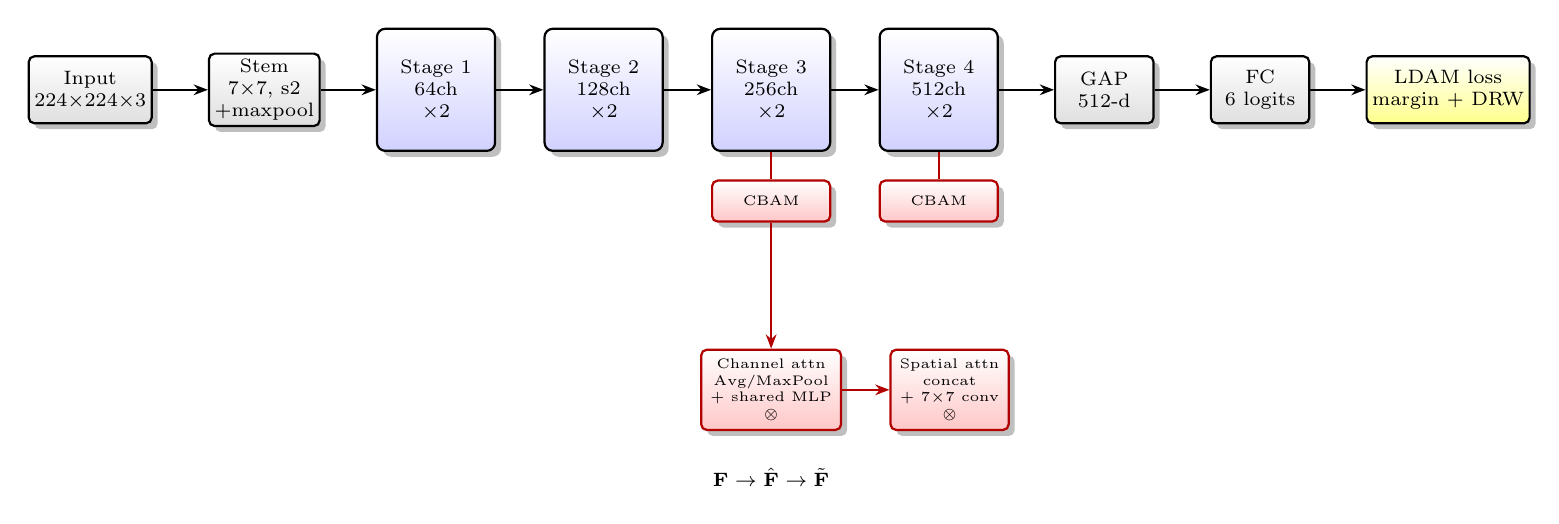
\begin{tikzpicture}[
			box/.style={rectangle,draw,thick,rounded corners=2pt,minimum height=0.85cm,minimum width=1.25cm,font=\scriptsize,align=center,inner sep=2pt,top color=white,bottom color=gray!25,drop shadow},
			stg/.style={rectangle,draw,thick,rounded corners=3pt,minimum height=1.55cm,minimum width=1.5cm,font=\scriptsize,align=center,top color=white,bottom color=blue!18,drop shadow},
			attnb/.style={rectangle,draw=red!70!black,thick,rounded corners=2pt,minimum height=0.52cm,minimum width=1.5cm,font=\tiny,align=center,top color=white,bottom color=red!22,drop shadow},
			lbl/.style={font=\scriptsize},
			arr/.style={-{Stealth[length=1.8mm]},thick},
		]
			% ---- main pipeline ----
			\node[box] (in) {Input\\$224{\times}224{\times}3$};
			\node[box,right=0.7cm of in] (stem) {Stem\\$7{\times}7$, s2\\+maxpool};
			\node[stg,right=0.7cm of stem] (s1) {Stage 1\\$64$ch\\$\times2$};
			\node[stg,right=0.6cm of s1] (s2) {Stage 2\\$128$ch\\$\times2$};
			\node[stg,right=0.6cm of s2] (s3) {Stage 3\\$256$ch\\$\times2$};
			\node[stg,right=0.6cm of s3] (s4) {Stage 4\\$512$ch\\$\times2$};
			\node[box,right=0.7cm of s4] (gap) {GAP\\$512$-d};
			\node[box,right=0.7cm of gap] (fc) {FC\\$6$ logits};
			\node[box,right=0.7cm of fc,bottom color=yellow!45] (loss) {LDAM loss\\margin $+$ DRW};
			\draw[arr] (in)--(stem);
			\draw[arr] (stem)--(s1);
			\draw[arr] (s1)--(s2);
			\draw[arr] (s2)--(s3);
			\draw[arr] (s3)--(s4);
			\draw[arr] (s4)--(gap);
			\draw[arr] (gap)--(fc);
			\draw[arr] (fc)--(loss);
			% ---- CBAM tags on stages 3,4 ----
			\node[attnb,below=0.35cm of s3] (a3) {CBAM};
			\node[attnb,below=0.35cm of s4] (a4) {CBAM};
			\draw[thick,red!70!black] (s3.south)--(a3.north);
			\draw[thick,red!70!black] (s4.south)--(a4.north);
			% ---- CBAM module detail (bottom) ----
			\node[attnb,below=1.6cm of a3] (cdet) {Channel attn\\Avg/MaxPool\\$+$ shared MLP\\$\otimes$};
			\node[attnb,right=0.6cm of cdet] (sdet) {Spatial attn\\concat\\$+$ $7{\times}7$ conv\\$\otimes$};
			\draw[arr,red!70!black] (a3.south)--(cdet.north);
			\draw[arr,red!70!black] (cdet)--(sdet);
			\node[lbl,below=0.35cm of cdet] (clbl) {$\mathbf{F}\rightarrow\hat{\mathbf{F}}\rightarrow\tilde{\mathbf{F}}$};
		\end{tikzpicture}}
		\caption{The overall architecture of CSAR-Net. A ResNet18 backbone (Module 1) extracts hierarchical features through four residual stages; CBAM (Module 2) is injected into stages 3 and 4 for label-agnostic feature refinement (its channel and spatial sub-modules are shown at the bottom); the classifier produces six logits, on top of which the LDAM loss (Module 3) performs label-dependent cost-sensitive calibration during training only.}
		\label{fig:arch}
	\end{figure}

	\subsection{Module 1 --- Feature extraction backbone (ResNet18)}
	\label{sec:backbone}
	\par{
		The backbone is the standard ResNet18 \citep{he2016deep}, chosen for its balance of capacity and deployment cost on an industrial inspection line. Its stem is a $7\times7$ convolution with stride 2 followed by batch normalization, ReLU, and a $3\times3$ max-pooling with stride 2; the body is four residual stages with channel counts $64/128/256/512$, each containing two basic residual blocks. A basic block learns a residual function
		\begin{equation}
			\mathbf{y}=\mathrm{ReLU}\bigl(\mathcal{F}(\mathbf{x};\{W_i\})+\mathbf{x}\bigr),
		\end{equation}
		where $\mathcal{F}(\mathbf{x};\{W_i\})$ is a stack of two $3\times3$ convolutions with batch normalization, and the identity skip $\mathbf{x}$ (or a $1\times1$ projection when the dimensions change) eases optimization \citep{he2016deep}. For $224\times224$ input the four stages produce feature maps of spatial size $56$, $28$, $14$, and $7$, respectively, and a global average pooling layer collapses the final $7\times7\times512$ map into a 512-dimensional vector.
	}

	\subsection{Module 2 --- Feature-layer attention refinement (CBAM)}
	\label{sec:cbam}
	\par{
		Raw features extracted by the backbone need enhancement because real magnetic tile defects are visually confusable. CBAM \citep{woo2018cbam} refines a feature map by sequentially reweighting its channels and spatial locations. It is injected into the residual blocks of stages 3 and 4 (256/512 channels), after the second convolution and before the residual addition, so that the attention reweights only the residual branch while the identity skip remains intact:
		\begin{equation}
			\hat{\mathbf{F}}=\sigma\bigl(M_c(\mathbf{F})\bigr)\otimes\mathbf{F},\qquad
			\tilde{\mathbf{F}}=\sigma\bigl(M_s(\hat{\mathbf{F}})\bigr)\otimes\hat{\mathbf{F}},
		\end{equation}
		where $\otimes$ denotes element-wise multiplication and $\sigma$ is the sigmoid. The channel attention map is
		\begin{equation}
			M_c(\mathbf{F})=\mathrm{MLP}\bigl(\mathrm{AvgPool}(\mathbf{F})\bigr)+\mathrm{MLP}\bigl(\mathrm{MaxPool}(\mathbf{F})\bigr),
		\end{equation}
		with a shared two-layer MLP of reduction ratio 16, and the spatial attention map is
		\begin{equation}
			M_s(\hat{\mathbf{F}})=\mathrm{Conv}_{7\times7}\bigl(\,[\,\overline{\hat{\mathbf{F}}};\ \widehat{\hat{\mathbf{F}}}\,]\,\bigr),
		\end{equation}
		where $\overline{\cdot}$ and $\widehat{\cdot}$ are the channel-wise mean and max statistics concatenated along the channel axis. Two properties of CBAM matter for the rest of this paper. First, it is \emph{label-agnostic}: the attention weights depend only on the input features, so the module behaves identically in training and inference. Second, it is \emph{cheap}: as quantified in Section \ref{sec:complexity}, the two CBAM blocks add fewer than $1\%$ parameters to the backbone.
	}

	\subsection{Module 3 --- Loss-layer cost-sensitive calibration (LDAM)}
	\label{sec:ldam}
	\par{
		The cost-sensitive signal is placed in the loss layer, not in the feature path. LDAM \citep{cao2019learning} assigns each class a margin that decays with its sample count
		\begin{equation}
			\Delta_c=\frac{C}{n_c^{1/4}},
		\end{equation}
		and subtracts it from the true-class logit during training, so that minority classes obtain a larger classification margin and a wider decision boundary. Here $C$ is the margin coefficient ($0.5$ unless stated otherwise) and $n_c$ is the number of training samples of class $c$. In its full form LDAM further multiplies the cross-entropy by class-balanced weights based on the effective number of samples \citep{cui2019class},
		\begin{equation}
			w_c=\frac{1-\beta}{1-\beta^{\,n_c}},\qquad\beta=0.9999,
		\end{equation}
		where $\beta$ controls how quickly the effective count saturates. The full LDAM loss composes the two into a single training objective
		\begin{equation}
			\mathcal{L}_{\text{LDAM}}(z,y)=w_y\Bigl(-\log\frac{e^{z_y-\Delta_y}}{e^{z_y-\Delta_y}+\sum_{j\neq y}e^{z_j}}\Bigr),
			\label{eq:ldam}
		\end{equation}
		where $z_y$ is the true-class logit: the margin $\Delta_y$ is subtracted only from the true-class logit, and the class-balanced weight $w_y$ scales the whole sample. Because these two components (the margin and the reweighting) have opposite empirical effects on this small real dataset, we \emph{decompose} them in the ablation (Section \ref{sec:ablation}) by testing margin-only LDAM (no reweighting) and inverse-frequency-weighted cross-entropy (CS-CE, no margin) separately.
	}

	\subsection{Module stitching --- the decoupling principle}
	\label{sec:stitching}
	\par{
		The central design decision of CSAR-Net is \emph{decoupling}: CBAM is a label-agnostic operator in the feature layer, whereas LDAM is a label-dependent calibration that acts only on the training objective and vanishes at inference. The two modules are stitched together by \emph{layer}, so that each does the job it is structurally suited to. The intuition, made concrete in Section \ref{sec:discussion}, is that feature attention sharpens the discriminative features of rare classes, whereas loss calibration re-weights the training objective; the decoupling exposes which of these two effects actually helps on small real data (the former) and which over-corrects (the latter). Fig.~\ref{fig:mechanism} (left) illustrates this decoupled arrangement.
	}

	\subsection{Counter-design --- the coupled CS-CBAM}
	\label{sec:cscbam}
	\par{
		To test whether the decoupling is necessary rather than incidental, we implement a \emph{coupled} counter-design, CS-CBAM, which injects the class prior $\lambda\log(N/n_c)$ directly into the attention logits (before the sigmoid) of the CBAM block, so that tail-class samples receive larger attention weights during training. As shown in Fig.~\ref{fig:mechanism} (right) and quantified in Section \ref{sec:ablation}, this coupling breaks train/inference consistency and collapses the classifier to the majority class: during training the label is known and the network learns the shortcut ``large attention response $=$ tail class,'' but at inference the label is unknown and the shortcut fails. The contrast between the decoupled CSAR-Net and the coupled CS-CBAM isolates the correct placement of the cost signal.
	}

	\begin{figure}[pos=htbp]
		\centering
		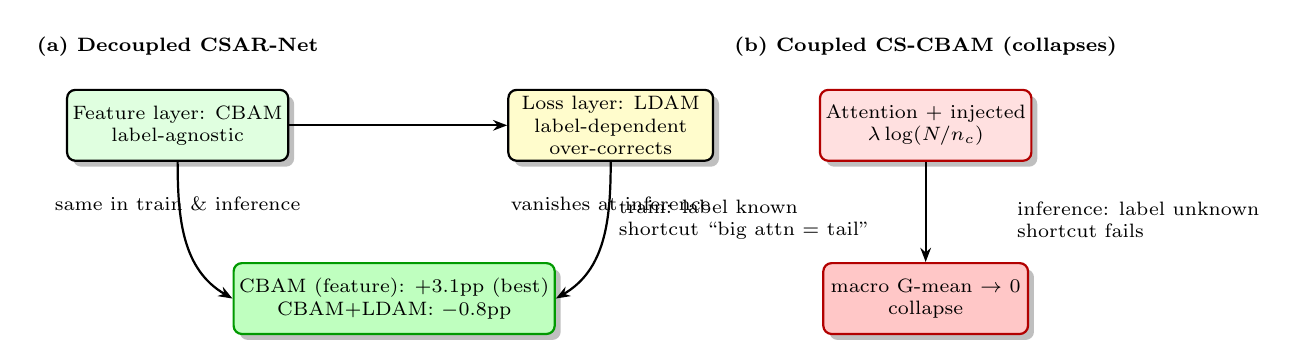
\begin{tikzpicture}[
			mod/.style={rectangle,draw,thick,rounded corners=3pt,minimum height=0.9cm,minimum width=2.6cm,font=\scriptsize,align=center,inner sep=2pt,drop shadow},
			lab/.style={font=\scriptsize,align=left},
			arr/.style={-{Stealth[length=1.8mm]},thick},
		]
			% ---- (a) decoupled ----
			\node[lab] at (0,0) {\textbf{(a) Decoupled CSAR-Net}};
			\node[mod,fill=green!12] (f) at (0,-1.0) {Feature layer: CBAM\\label-agnostic};
			\node[mod,fill=yellow!20] (l) at (5.5,-1.0) {Loss layer: LDAM\\label-dependent\\over-corrects};
			\node[lab] at (0,-2.0) {same in train \& inference};
			\node[lab] at (5.5,-2.0) {vanishes at inference};
			\node[mod,fill=green!25,draw=green!60!black] (ok) at (2.75,-3.2) {CBAM (feature): $+$3.1pp (best)\\CBAM$+$LDAM: $-$0.8pp};
			\draw[arr] (f)--(l);
			\draw[arr] (f.south) to[out=-90,in=150] (ok.west);
			\draw[arr] (l.south) to[out=-90,in=30] (ok.east);

			% ---- (b) coupled ----
			\node[lab] at (9.5,0) {\textbf{(b) Coupled CS-CBAM (collapses)}};
			\node[mod,fill=red!12,draw=red!70!black] (cf) at (9.5,-1.0) {Attention $+$ injected\\$\lambda\log(N/n_c)$};
			\node[lab] at (7.2,-2.2) {train: label known\\shortcut ``big attn $=$ tail''};
			\node[lab] at (12.2,-2.2) {inference: label unknown\\shortcut fails};
			\node[mod,fill=red!22,draw=red!70!black] (bad) at (9.5,-3.2) {macro G-mean $\to$ 0\\collapse};
			\draw[arr] (cf.south) to[out=-90,in=90] (bad.north);
		\end{tikzpicture}
		\caption{The mechanism contrast. (a) The decoupled CSAR-Net places CBAM (label-agnostic) in the feature layer and LDAM (label-dependent) in the loss layer, so the two effects can be isolated: CBAM is the robust gain ($+$3.1pp), whereas LDAM over-corrects and stacking it on CBAM dilutes the gain to $-$0.8pp. (b) The coupled CS-CBAM injects the class prior into the attention logits, creating a train/inference distribution shift that collapses the classifier to the majority class.}
		\label{fig:mechanism}
	\end{figure}

	\begin{table}[pos=htbp]
		\small
		\caption{Training procedure of CSAR-Net and its ablation variants. The three flags \texttt{use\_cbam}, \texttt{use\_ldam}, and \texttt{use\_cs} select the module ablations in Section \ref{sec:ablation}.}
		\label{alg:train}
		\centering
		\begin{tabular}{@{}l l@{}}
			\multicolumn{2}{@{}l}{\textbf{Algorithm 1}~ Training CSAR-Net (and its ablations)}\\[3pt]
			\multicolumn{2}{@{}l}{Input: long-tailed dataset $\mathcal{D}$; backbone $f_\theta$ (ResNet18); flags \texttt{use\_cbam}, \texttt{use\_ldam}, \texttt{use\_cs}.}\\[3pt]
			1. & Build $f_\theta$; if \texttt{use\_cbam}, inject CBAM into stages 3--4 (after the 2nd conv, before the residual add).\\
			2. & \textbf{for} each epoch \textbf{do}\\
			3. & \quad \textbf{for} each mini-batch $(\mathbf{x}, y)$ \textbf{do}\\
			4. & \quad\quad $z \leftarrow g_\theta(\mathbf{x})$ \hfill (forward logits)\\
			5. & \quad\quad \textbf{if} \texttt{use\_cs}: add $\lambda\log(N/n_y)$ to the CBAM attention logits (CS-CBAM).\\
			6. & \quad\quad \textbf{if} \texttt{use\_ldam}: $z_y \leftarrow z_y-\Delta_y$; $\ell \leftarrow w_y\,\mathrm{CE}(z,y)$ \hfill (Eq.~\eqref{eq:ldam})\\
			7. & \quad\quad \textbf{else}: $\ell \leftarrow \mathrm{CE}(z,y)$\\
			8. & \quad\quad $\theta \leftarrow \mathrm{Adam}(\theta,\nabla_\theta \ell)$\\
			9. & Evaluate macro G-mean on the test split; repeat for seeds $\{42,123,2024\}$ and report mean$\pm$std.\\
		\end{tabular}
	\end{table}

	\subsection{Complexity analysis}
	\label{sec:complexity}
	\par{
		CSAR-Net adds a negligible computational footprint to its backbone. The plain ResNet18 has 11.18M parameters; injecting CBAM into stages 2, 3, and 4 adds $0.004$, $0.016$, and $0.065$M parameters, respectively, so the full CSAR-Net (stages 3 and 4) has 11.26M parameters, an overhead of only $0.7\%$ (Table \ref{tbl:complexity}). The LDAM loss and the CS-CBAM bias term add no parameters, since both are functions of the class counts rather than learnable weights. Because CBAM is inserted only in stages 3 and 4, the added FLOPs are concentrated on the smaller ($14\times14$ and $7\times7$) feature maps, keeping the inference-time overhead small: the two CBAM blocks contribute roughly $0.07$M and $0.14$M multiply--accumulate operations, three orders of magnitude below the $\approx$1.8G MACs of the ResNet18 forward pass. The network can therefore be served at the same latency as the plain backbone, which matters for an edge-deployed inspection line.

		\begin{table}[pos=htbp]
			\footnotesize
			\caption{Parameter budget of CSAR-Net. CBAM adds $0.7\%$ parameters; LDAM and the CS-CBAM bias add none.}
			\label{tbl:complexity}
			\centering
			\begin{tabular}{lcc}
				\hline
				\textbf{Component} & \textbf{Params (M)} & \textbf{Note} \\ \hline
				Plain ResNet18 (6-class FC) & 11.18 & baseline \\
				$+$CBAM stage 3 & $+$0.016 & channel MLP ($r{=}16$) $+$ spatial $7{\times}7$, 2 blocks \\
				$+$CBAM stage 4 & $+$0.065 & same, 2 blocks \\
				CSAR-Net & 11.26 & $+0.7\%$ overhead \\
				$+$LDAM / $+$CS-CBAM & $+$0 & functions of class counts \\ \hline
			\end{tabular}
		\end{table}
	}

	%% 4. Experiments
	\section{Experiments}
	\label{sec:exp}

	\subsection{Dataset and experimental setup}
	\label{sec:dataset}
	\par{
		Experiments use the real industrial dataset MTSD (Magnetic Tile Surface Defects) \citep{huang2020surface}, comprising 1344 grayscale magnetic tile surface images in 6 classes: defect-free (Free) 952, blowhole 115, uneven 103, break 85, crack 57, and fray 32, a natural imbalance ratio of about 30:1. Fig.~\ref{fig:samples} shows representative samples of the six classes. The images are captured in a real inspection setting, so their long-tailed distribution, illumination variation, and defect-morphology diversity are all authentic. Image short sides range from 103 to 392 pixels; all images are resized to $224\times224$ and the grayscale channel is replicated into three channels. A class-stratified random train/test split (80\%/20\%, split seed fixed for fair comparison) yields per-class training counts of about 761/92/82/68/46/26. The optimizer is Adam (lr $=10^{-3}$, weight decay $=10^{-4}$) with cosine annealing over 40 epochs, and random horizontal/vertical flip augmentation. Every configuration is run once per random seed (42, 123, 2024), and results are reported as mean$\pm$std. Table \ref{tbl:hyper} consolidates the full configuration; every ablation in Section \ref{sec:ablation} reuses exactly this recipe except for the single factor being varied, which is what makes the ablation controlled.
	}

	\begin{figure}[pos=htbp]
		\centering
		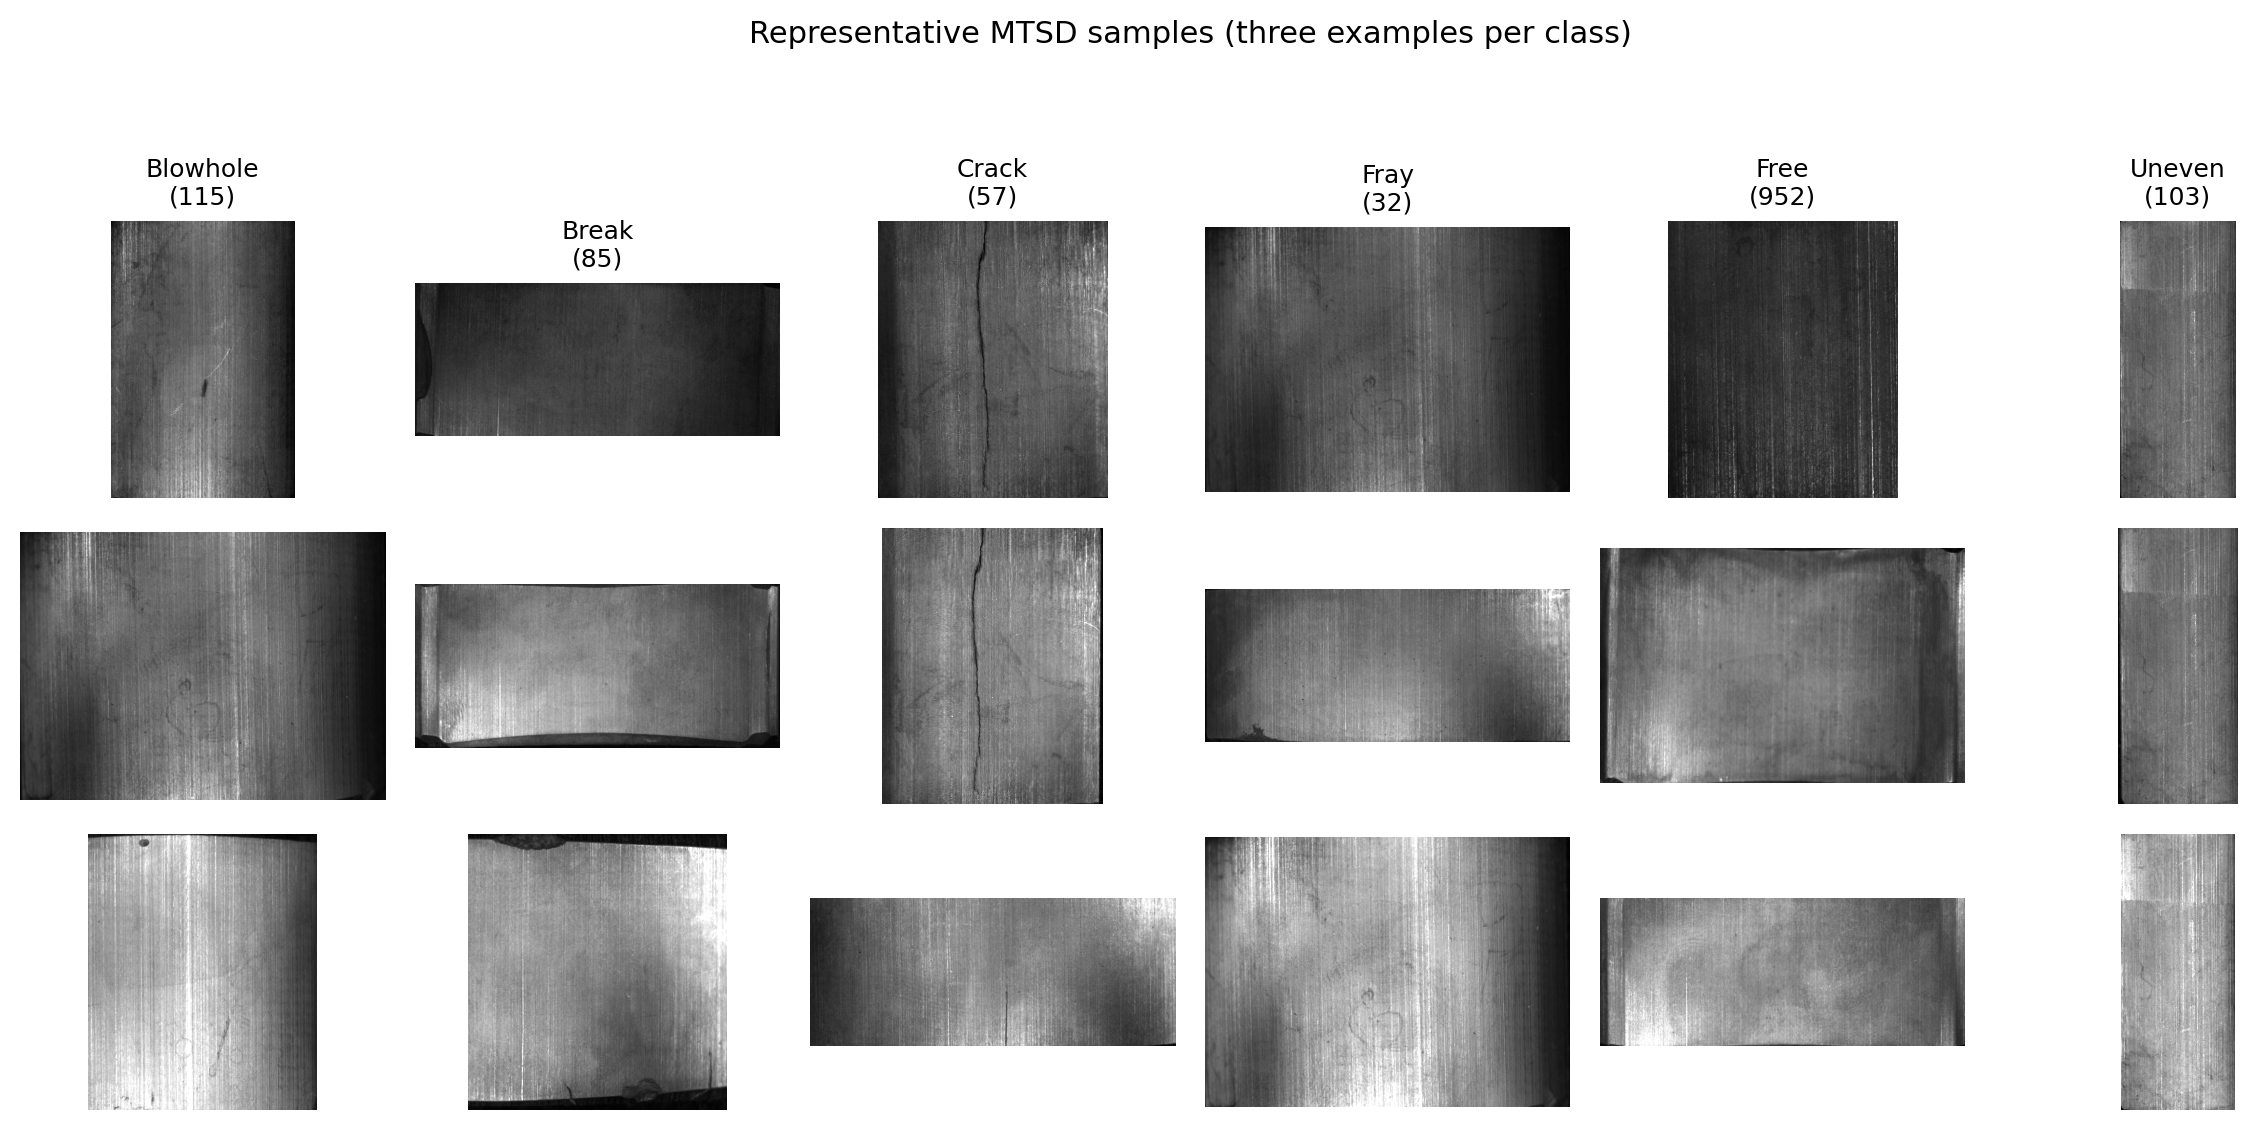
\includegraphics[width=0.95\textwidth]{./figures/dataset_samples.png}
		\caption{Representative MTSD samples (three examples per class). The six classes span a natural imbalance of about 30:1 from defect-free (952) to fray (32), with authentic intra-class variation in defect shape, scale, and illumination.}
		\label{fig:samples}
	\end{figure}

	\begin{table}[pos=htbp]
		\footnotesize
		\caption{Training configuration. All ablations reuse this recipe except for the single factor under study.}
		\label{tbl:hyper}
		\centering
		\setlength{\tabcolsep}{2pt}
		\begin{tabular}{ll}
			\hline
			\textbf{Item} & \textbf{Value} \\ \hline
			Input size & $224{\times}224{\times}3$ (grayscale replicated) \\
			Train/test split & class-stratified 80\%/20\%, fixed split seed \\
			Optimizer & Adam (lr $10^{-3}$, weight decay $10^{-4}$) \\
			Learning-rate schedule & cosine annealing \\
			Epochs & 40 \\
			Batch size & 32 \\
			Augmentation & random horizontal/vertical flip \\
			CBAM reduction ratio & $r=16$ \\
			LDAM margin & $C=0.5$, $\beta=0.9999$ \\
			Seeds & 42, 123, 2024 \\
			cuDNN & deterministic (benchmark off) \\ \hline
		\end{tabular}
	\end{table}

	\begin{table}[pos=htbp]
		\footnotesize
		\caption{Per-class composition of MTSD and the class-stratified 80\%/20\% split used here. The imbalance ratio $N/n_c$ grows from $1$ (defect-free) to $\approx$30 (fray).}
		\label{tbl:data}
		\centering
		\begin{tabular}{lcccc}
			\hline
			\textbf{Class} & \textbf{Total} & \textbf{Train} & \textbf{Test} & \textbf{$N/n_c$} \\ \hline
			Defect-free (Free) & 952 & 761 & 191 & 1.0 \\
			Blowhole & 115 & 92 & 23 & 8.3 \\
			Uneven & 103 & 82 & 21 & 9.2 \\
			Break & 85 & 68 & 17 & 11.2 \\
			Crack & 57 & 46 & 11 & 16.7 \\
			Fray & 32 & 26 & 6 & 29.8 \\ \hline
		\end{tabular}
	\end{table}

	\subsection{Evaluation metrics}
	\label{sec:metrics}
	\par{
		Under long-tailed distributions, average accuracy is biased toward the majority class and can hide the misses of rare defects; the CE baseline already reaches 0.905 average accuracy while recalling only 0.490 of the break class. We therefore adopt \emph{macro G-mean}, the geometric mean of per-class recalls, as the primary metric: it penalizes the weakest class and matches the goal of protecting rare defects. We also report macro F1, the arithmetic mean of the per-class harmonic means of precision and recall,
\begin{equation}
	\text{macro-F1}=\frac{1}{K}\sum_{c=1}^{K}\frac{2\,\mathrm{Precision}_c\cdot\mathrm{Recall}_c}{\mathrm{Precision}_c+\mathrm{Recall}_c},
	\label{eq:macroF1}
\end{equation}
and the Matthews correlation coefficient (MCC), a single chance-corrected scalar summarizing the whole confusion matrix, together with per-class recall, to give a complete picture.
	}

	\subsection{Main results}
	\label{sec:mainres}
	\par{
		Table \ref{tbl:main} reports the main results. Three observations stand out. First, CBAM is a stable gain: adding it to the CE baseline raises macro G-mean by $+$3.1pp (0.752 to 0.782) and attains the lowest variance among all configurations (0.039 vs.\ 0.060 for CE), indicating that attention genuinely enhances real complex defect features rather than merely adding capacity. Second, LDAM alone degrades: the full LDAM loss drops macro G-mean by 8.6pp with a large variance (0.120), which reflects the over-correction risk of aggressive reweighting on small samples. Third, stacking LDAM on CBAM does not combine their benefits: CSAR-Net (CBAM$+$LDAM) reaches 0.744, below both CBAM (0.782) and CE (0.752), so the loss-layer calibration dilutes the attention gain by 3.9pp. The coupled CS-CBAM collapses, confirming that the cost signal must not be injected into attention.
	}

	\begin{table}[pos=htbp]
		\footnotesize
		\caption{Main results on MTSD (3 seeds, mean$\pm$std). CBAM stably improves macro G-mean by $+$3.1pp; LDAM alone degrades by 8.6pp; stacking LDAM on CBAM dilutes the attention gain.}
		\label{tbl:main}
		\centering
		\begin{tabular}{lccccc}
	\hline
	\textbf{Method} & \textbf{G-mean} & \textbf{Acc} & \textbf{Macro F1} & \textbf{MCC} & \textbf{vs CE} \\ \hline
	ResNet18 (CE) & 0.7515$\pm$0.0598 & 0.9046$\pm$0.0274 & 0.809 & 0.790 & --- \\
	ResNet18 $+$ CBAM & 0.7822$\pm$0.0393 & 0.9133$\pm$0.0018 & 0.821 & 0.812 & $+$3.1pp \\
	ResNet18 $+$ LDAM & 0.6658$\pm$0.1197 & 0.6543$\pm$0.1735 & 0.578 & 0.478 & $-$8.6pp \\
	\textbf{CSAR-Net} & \textbf{0.7437$\pm$0.0526} & 0.8116$\pm$0.0673 & 0.705 & 0.647 & \textbf{$-$0.8pp} \\
	CS-CBAM & 0.0000$\pm$0.0000 & 0.6865$\pm$0.0333 & 0.141 & $-$0.006 & collapse \\
	\hline
	\end{tabular}
	\end{table}

	\subsection{Statistical robustness across seeds}
	\label{sec:stats}
	\par{
		Because the dataset is small, seed-to-seed variance is a first-order concern, and the paper's claims should be read against it. Table \ref{tbl:seeds} reports the per-seed macro G-mean behind every mean in Table \ref{tbl:main}. Two properties support the main conclusion. First, CBAM is the most \emph{stable} configuration: its across-seed standard deviation (0.039) is the lowest among the four trained variants, and it is higher than the CE baseline in 2 of 3 seeds (0.7295 vs.\ 0.6801 and 0.8239 vs.\ 0.7478) while lower in the third (0.7931 vs.\ 0.8265); the mean gain of $+3.1$pp therefore reflects a genuine reduction in variance rather than a single favorable seed. Second, the failures are \emph{deterministic rather than noisy}: CS-CBAM collapses to a macro G-mean of $\approx$0 in all three seeds, and LDAM's large standard deviation (0.120) reflects its instability (0.542, 0.828, and 0.628 across seeds) rather than a uniformly weak performance. With only three seeds a formal paired significance test has low power: the paired difference CBAM$-$CE is $+0.031\pm0.057$ (std of the differences), so the improvement is indicative but not statistically conclusive. We therefore report effect sizes and per-seed values transparently rather than claiming significance, and defer confirming the gain at conventional levels to a larger-seed protocol in future work.
	}

	\begin{table}[pos=htbp]
		\footnotesize
		\caption{Per-seed macro G-mean behind the means in Table \ref{tbl:main}. CBAM is the most stable configuration; CS-CBAM collapses identically in every seed.}
		\label{tbl:seeds}
		\centering
		\setlength{\tabcolsep}{3pt}
		\begin{tabular}{lccccc}
		\hline
		\textbf{Method} & \textbf{42} & \textbf{123} & \textbf{2024} & \textbf{mean} & \textbf{std} \\ \hline
		ResNet18 (CE) & 0.6801 & 0.8265 & 0.7478 & 0.7515 & 0.0598 \\
		ResNet18 $+$ CBAM & 0.7295 & 0.7931 & 0.8239 & 0.7822 & 0.0393 \\
		ResNet18 $+$ LDAM & 0.5417 & 0.8276 & 0.6280 & 0.6658 & 0.1197 \\
		CSAR-Net & 0.6935 & 0.8163 & 0.7213 & 0.7437 & 0.0526 \\
		CS-CBAM & 0.0000 & 0.0001 & 0.0000 & 0.0000 & 0.0000 \\
		\hline
		\end{tabular}
	\end{table}

	\subsection{Per-class recall}
	\label{sec:perclass}
	\par{
		Table \ref{tbl:class} reports per-class recall. Under the CE baseline the hardest class is break (0.490): the difficulty of real defects arises not only from frequency bias but also from visual confusability among defect morphologies. CBAM improves the costly and confusable classes(break 0.490 to 0.549, $+$5.9pp; blowhole 0.768 to 0.841, $+$7.3pp; uneven 0.746 to 0.794, $+$4.8pp)while leaving crack and the defect-free recall (0.983 to 0.977) nearly intact, which is why its macro G-mean is the best. In contrast, stacking LDAM on CBAM sacrifices exactly the classes that cost calibration is meant to protect: break recall falls back to 0.471 and defect-free recall drops to 0.838, so the overall macro G-mean falls below CE. This inversion (feature attention protects the rare class cheaply, whereas loss reweighting destroys it) is the paper's central empirical finding.
	}

	\begin{table}[pos=htbp]
		\footnotesize
		\caption{Per-class recall (3 seeds, mean). CBAM improves the costly classes while keeping defect-free recall nearly intact; adding LDAM drops break recall back below the baseline.}
		\label{tbl:class}
		\centering
		\begin{tabular}{lccc}
	\hline
	\textbf{Class (count)} & \textbf{CE} & \textbf{CBAM$+$CE} & \textbf{CSAR-Net} \\ \hline
	Blowhole (115) & 0.768 & 0.841 & 0.870 \\
	Break (85) & 0.490 & 0.549 & 0.471 \\
	Crack (57) & 0.788 & 0.788 & 0.727 \\
	Fray (32) & 0.889 & 0.833 & 0.833 \\
	Defect-free (952) & 0.983 & 0.977 & 0.838 \\
	Uneven (103) & 0.746 & 0.794 & 0.825 \\
	\hline
	\end{tabular}
	\end{table}

	\subsection{Ablation studies}
	\label{sec:ablation}
	\par{
		We conduct a decomposition-first ablation. Because CSAR-Net is a stitched network, the ablation asks two questions: \emph{(i) what does each module contribute, and (ii) where should each module be placed?} The first is answered by the module ablation (Table \ref{tbl:abl}); the second by the injection-position, sub-module, and margin-coefficient ablations (Tables \ref{tbl:ablpos}--\ref{tbl:ablC}).
	}

	\par{
		\emph{Module contribution} (Table \ref{tbl:abl}). Two diagnostics emerge. First, \emph{LDAM's degradation comes from both components, chiefly its class-balanced reweighting (DRW)}: margin-only LDAM without DRW reaches 0.7135 ($-$3.8pp vs.\ CE 0.7515), reweighting-only CS-CE reaches 0.7032 ($-$4.8pp), and the full LDAM (margin$+$DRW) is the worst at 0.6658 ($-$8.6pp): the margin and the reweighting are each harmful on this small dataset, and their combination is more harmful than either alone. Second, \emph{CS-CBAM collapses}: injecting the class prior into attention logits breaks train/inference consistency, a robust failure conclusion.
	}

	\begin{table}[pos=htbp]
		\footnotesize
		\caption{Module-contribution ablation (3 seeds, mean$\pm$std). LDAM degrades in both components, chiefly its class-balanced reweighting (DRW); feature-layer CBAM is the only robust gain.}
		\label{tbl:abl}
		\centering
		\begin{tabular}{lcc}
	\hline
	\textbf{Ablation} & \textbf{G-mean} & \textbf{vs CE} \\ \hline
	ResNet18 (CE baseline) & 0.7515$\pm$0.0598 & --- \\
	$+$CBAM (feature layer) & 0.7822$\pm$0.0393 & $+$3.1pp \\
	$+$LDAM (margin$+$DRW) & 0.6658$\pm$0.1197 & $-$8.6pp \\
	$+$LDAM (margin only) & 0.7135$\pm$0.0244 & $-$3.8pp \\
	$+$CS-CE (inverse-freq.) & 0.7032$\pm$0.1074 & $-$4.8pp \\
	\textbf{CSAR-Net ($+$CBAM$+$LDAM)} & \textbf{0.7437$\pm$0.0526} & \textbf{$-$0.8pp} \\
	$+$CS-CBAM (cost into attention) & 0.0000$\pm$0.0000 & collapse \\
	\hline
	\end{tabular}
	\end{table}

	\par{
		\emph{Injection position} (Table \ref{tbl:ablpos}). To locate where attention helps most, we inject CBAM into stage 2, stage 3, stage 4, and stages 3$+$4 (the CSAR-Net choice) under the CE loss. The gain is robust to injection position: stage 2 (0.794), stage 3 (0.787), and stages 3$+$4 (0.782) all clear the CE baseline (0.752) by 3--4pp, with their differences well within seed noise (std 0.03--0.05). Only stage 4 alone (0.699) is clearly worse, because its $7\times7$ maps leave too little spatial resolution for spatial attention to sharpen rare-defect features. We retain stages 3$+$4 as the CSAR-Net choice because it matches the best single-stage positions while covering the two deepest scales at which defects manifest.
	}

	\begin{table}[pos=htbp]
		\footnotesize
		\caption{CBAM injection position (CE loss, 3 seeds, mean$\pm$std). Stage 2, stage 3, and stages 3$+$4 all clear the baseline within noise; only stage 4 alone is clearly worse.}
		\label{tbl:ablpos}
		\centering
		\begin{tabular}{lcc}
			\hline
			\textbf{Position} & \textbf{G-mean} & \textbf{Acc} \\ \hline
			Stage 2 only & 0.7936$\pm$0.0536 & 0.9195$\pm$0.0213 \\
			Stage 3 only & 0.7870$\pm$0.0313 & 0.9157$\pm$0.0202 \\
			Stage 4 only & 0.6991$\pm$0.1003 & 0.8934$\pm$0.0299 \\
			Stage 3$+$4 (CSAR-Net) & 0.7822$\pm$0.0393 & 0.9133$\pm$0.0018 \\ \hline
		\end{tabular}
	\end{table}

	\par{
		\emph{Channel vs.\ spatial sub-module} (Table \ref{tbl:ablsub}). CBAM is itself a two-part module; we decompose it into channel-only and spatial-only variants to attribute its gain. Neither sub-module alone helps: channel-only (0.754) is within noise of CE (0.752), and spatial-only (0.742) is slightly below it. Only the series combination (0.782, $+$3.1pp) yields the full gain: channel reweighting first selects which feature maps matter, and spatial attention then localizes where, so neither step is sufficient alone. This justifies the ``convolutional block'' design of CBAM.
	}

	\begin{table}[pos=htbp]
		\footnotesize
		\caption{CBAM sub-module decomposition (stages 3$+$4, CE loss, 3 seeds, mean$\pm$std). Neither channel-only nor spatial-only clears the baseline; only their series combination yields the gain.}
		\label{tbl:ablsub}
		\centering
		\begin{tabular}{lcc}
			\hline
			\textbf{Variant} & \textbf{G-mean} & \textbf{Acc} \\ \hline
			Channel attention only & 0.7544$\pm$0.0385 & 0.9219$\pm$0.0080 \\
			Spatial attention only & 0.7415$\pm$0.0405 & 0.9145$\pm$0.0121 \\
			Channel $+$ spatial (CBAM) & 0.7822$\pm$0.0393 & 0.9133$\pm$0.0018 \\ \hline
		\end{tabular}
	\end{table}

	\par{
		\emph{Margin-coefficient sensitivity} (Table \ref{tbl:ablC}). We sweep the LDAM margin coefficient $C$ in two regimes. For margin-only LDAM (no reweighting), a small margin ($C=0.1$) is near-neutral (0.746 vs.\ CE 0.752), and larger margins degrade it mildly to $\approx$0.72 ($-$3pp): the margin component alone is not the main source of harm, but it is mildly negative at larger $C$. For the full CBAM$+$LDAM combination, the outcome is highly sensitive and non-monotonic in $C$: 0.769 ($C=0.1$), 0.765 ($C=0.3$), 0.744 ($C=0.5$), and 0.796 ($C=1.0$). The combination is therefore fragile: it swings by up to 5pp over a range where CBAM alone is stable, and at no $C$ does it robustly beat CBAM (0.782). This fragility, invisible at a single default value, is a further reason to prefer feature-layer attention.
	}

	\begin{table}[pos=htbp]
		\footnotesize
		\caption{Margin-coefficient sensitivity (3 seeds, mean$\pm$std G-mean). Margin-only LDAM degrades mildly at larger $C$; the CBAM$+$LDAM combination is non-monotonic and fragile in $C$.}
		\label{tbl:ablC}
		\centering
		\begin{tabular}{lcccc}
			\hline
			\textbf{Setting} & $C=0.1$ & $C=0.3$ & $C=0.5$ & $C=1.0$ \\ \hline
			LDAM margin only (no DRW) & 0.7455$\pm$0.0052 & 0.7185$\pm$0.0812 & 0.7135$\pm$0.0244 & 0.7189$\pm$0.0373 \\
			CSAR-Net (CBAM$+$LDAM) & 0.7692$\pm$0.0308 & 0.7646$\pm$0.0950 & 0.7437$\pm$0.0526 & 0.7955$\pm$0.0095 \\ \hline
		\end{tabular}
	\end{table}

	\subsection{Attention variant comparison}
	\label{sec:attn}
	\par{
		Table \ref{tbl:attn} compares attention variants under the CE loss. CBAM and SE both clear the baseline (0.782 and 0.782 vs.\ 0.752, $+$3.1pp and $+$3.0pp), while the lighter ECA (0.731) and CA (0.740) fall slightly below it. The gain is therefore not a universal property of any attention module but requires the fuller channel/spatial recalibration that CBAM and SE provide; CBAM is retained in CSAR-Net because it matches the best while being the most extensively ablated.
	}

	\begin{table}[pos=htbp]
		\footnotesize
		\caption{Attention variants (CE loss, 3 seeds, mean). CBAM and SE clear the CE baseline; the lighter ECA and CA do not, indicating the gain requires full channel/spatial recalibration.}
		\label{tbl:attn}
		\centering
		\begin{tabular}{lc}
	\hline
	\textbf{Attention} & \textbf{Macro G-mean} \\ \hline
	None (CE baseline) & 0.751 \\
	CBAM & 0.782 \\
	SE & 0.782 \\
	ECA & 0.731 \\
	CA & 0.740 \\
	\hline
	\end{tabular}
	\end{table}

	\subsection{Intermediate-representation analysis}
	\label{sec:repr}
	\par{
		\emph{Confusion matrices} (Fig.~\ref{fig:cm}): the baseline CE heavily misclassifies defect samples as defect-free or as a nearby defect class; CBAM$+$CE compresses this cross-class confusion and opens up the hardest break recall (0.490 to 0.549 across seeds), whereas adding LDAM does not further help (0.471 across seeds).
	}

	\begin{figure}[pos=htbp]
		\centering
		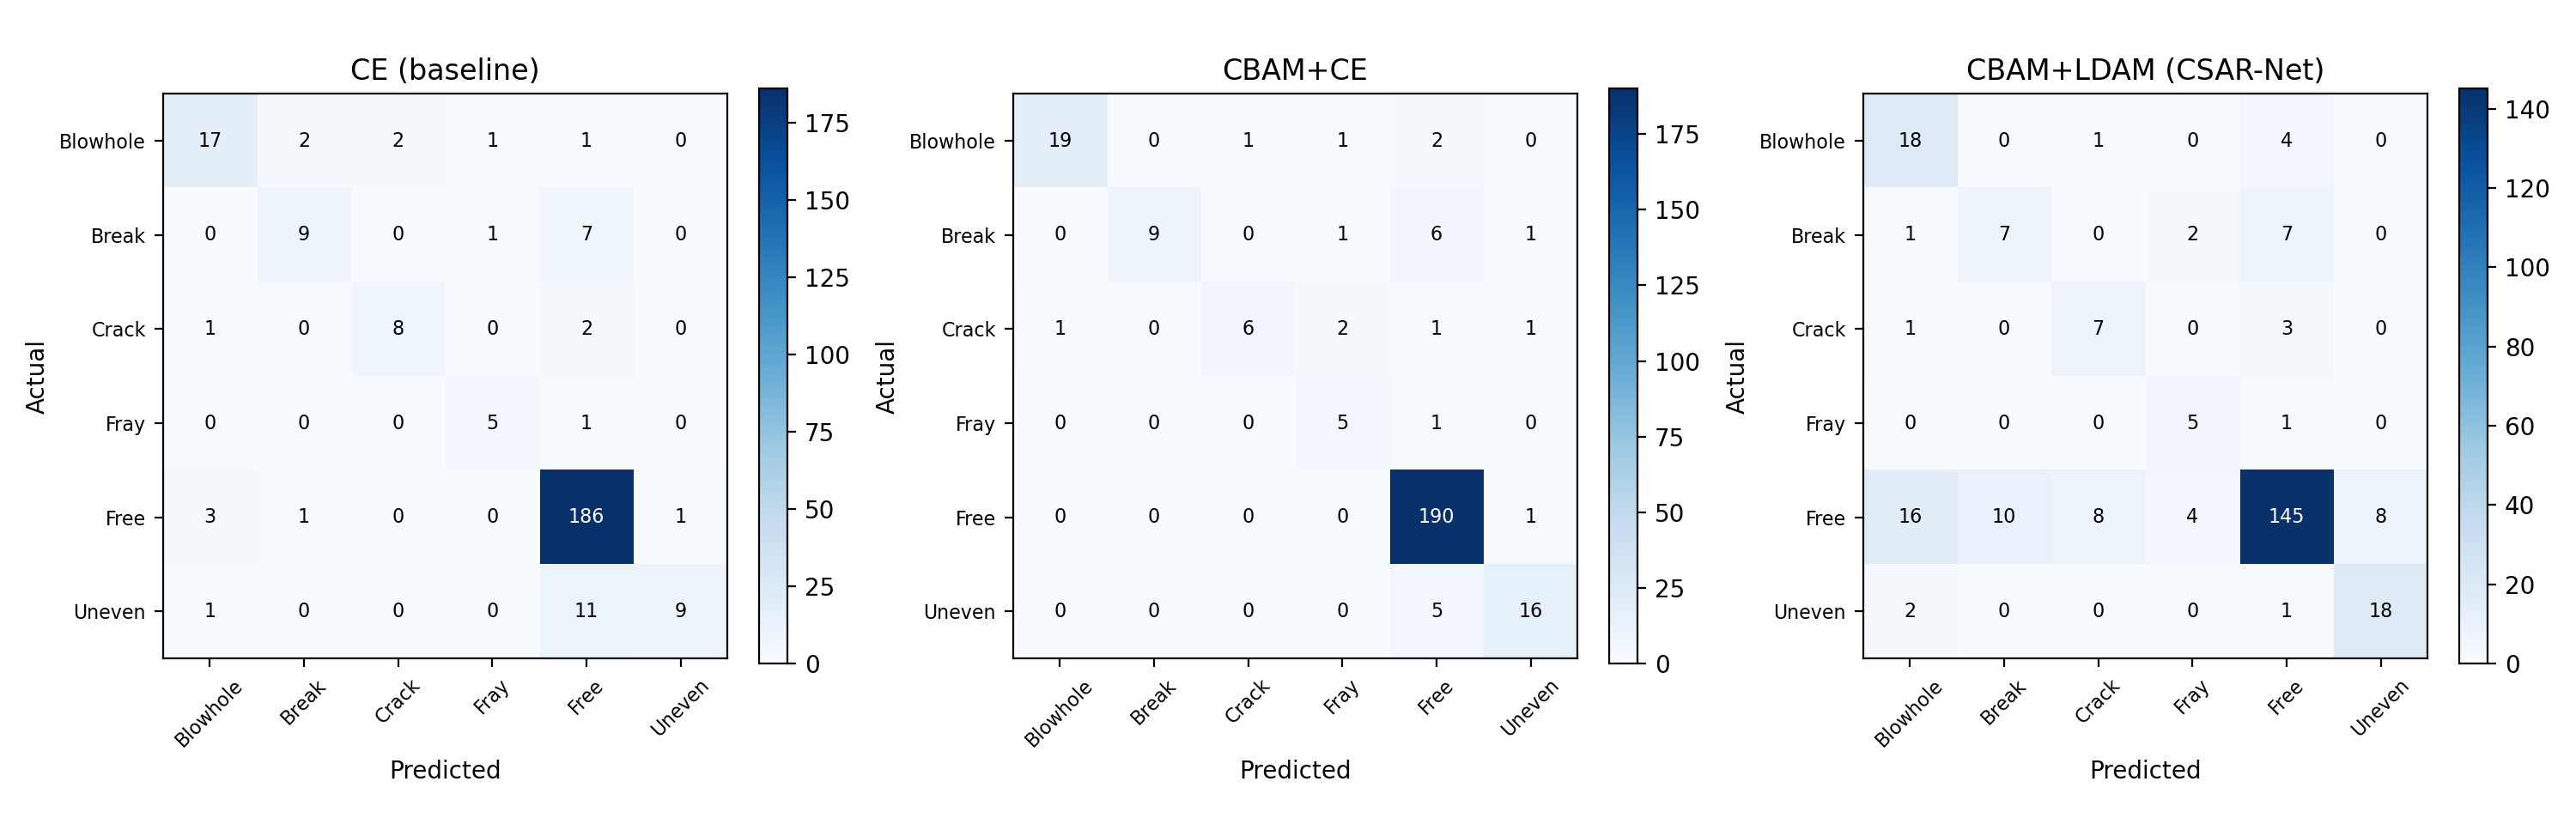
\includegraphics[width=0.9\textwidth]{./figures/confusion_mt.png}
		\caption{Confusion matrices of the CE baseline (left), CBAM$+$CE (middle), and CSAR-Net (right) on the magnetic tile test set (representative run).}
		\label{fig:cm}
	\end{figure}

	\par{
		\emph{Training curves} (Fig.~\ref{fig:train}) record CS-CBAM's collapse: its G-mean approaches 0 from the start of training, and the classifier degenerates into predicting the majority class (defect-free) for nearly all samples, providing direct evidence that the cost signal must not be injected into label-agnostic attention.
	}

	\begin{figure}[pos=htbp]
		\centering
		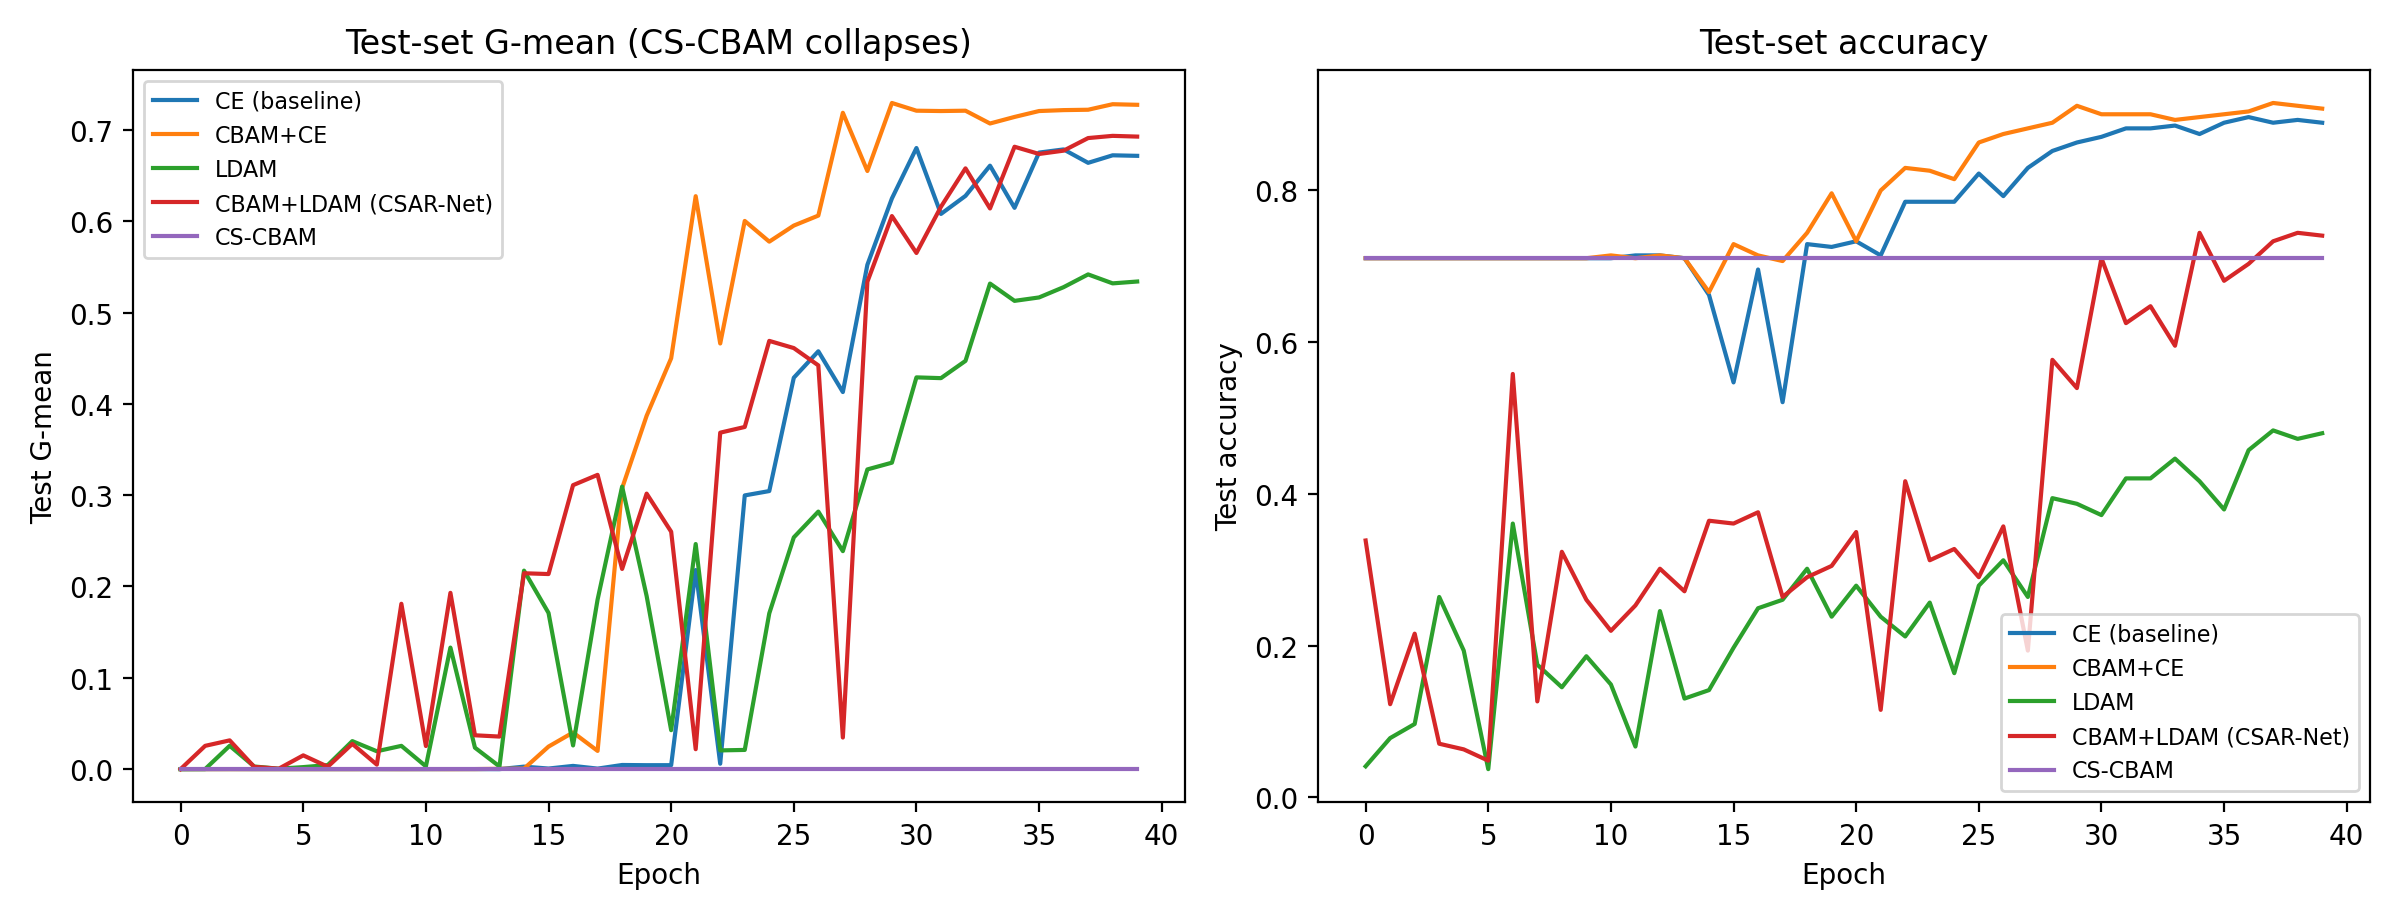
\includegraphics[width=0.9\textwidth]{./figures/training_mt.png}
		\caption{Test-set G-mean (left) and accuracy (right) over epochs. CS-CBAM's G-mean approaches 0 from the start.}
		\label{fig:train}
	\end{figure}

	\par{
		\emph{Feature separability} (Fig.~\ref{fig:tsne}): t-SNE \citep{maaten2008visualizing} shows the feature space learned by CBAM is more separable than the CE baseline (defect-class clusters more compact), confirming that CBAM's gain comes from enhanced feature discriminability; class-activation visualization such as Grad-CAM \citep{selvaraju2017grad} offers a complementary, instance-level view of which image regions drive the decision.
	}

	\begin{figure}[pos=htbp]
		\centering
		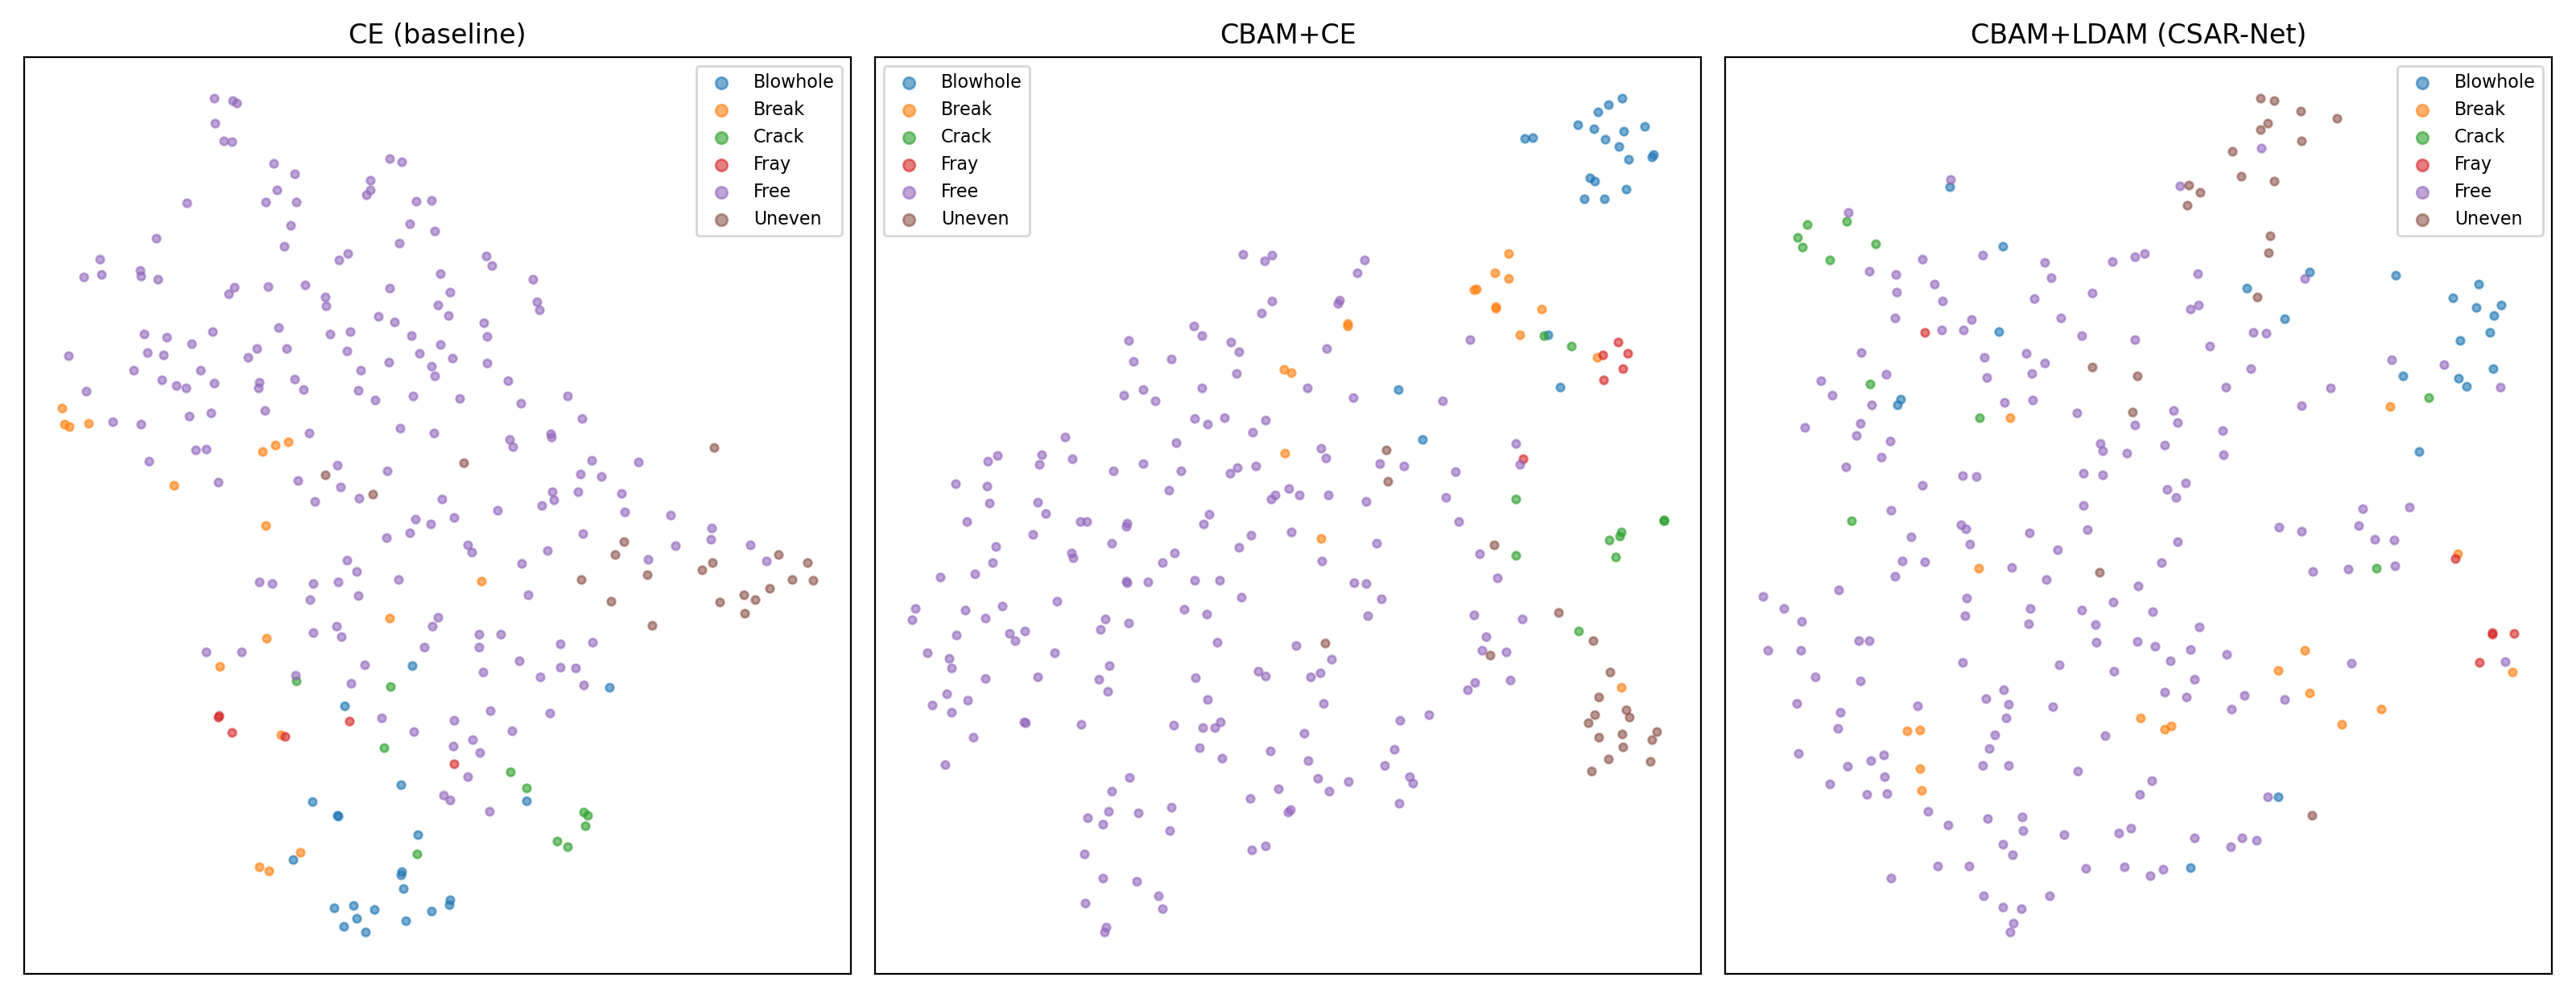
\includegraphics[width=0.9\textwidth]{./figures/tsne_mt.png}
		\caption{Penultimate-layer feature t-SNE of the CE baseline (left), CBAM$+$CE (middle), and CSAR-Net (right).}
		\label{fig:tsne}
	\end{figure}

	%% 5. Discussion
	\section{Discussion}
	\label{sec:discussion}

	\subsection{Why CBAM works: the complexity of real defect features}
	\par{
		Real magnetic tile defect images have complex textures, varying illumination, and mutually confusable morphologies (break vs.\ crack, blowhole vs.\ uneven). The raw features of a ResNet18 backbone then need enhancement, and CBAM's channel$+$spatial recalibration sharpens discriminative features, improving the costly classes break ($+$5.9pp), blowhole ($+$7.3pp), and uneven ($+$4.8pp) while leaving crack and the defect-free recall nearly intact. That attention helps precisely when features are complex, rather than uniformly, suggests that the value of attention depends on input feature complexity. The finding that SE matches CBAM while the lighter ECA and CA fall short further confirms that the gain requires sufficient recalibration capacity, not merely the presence of an attention module.
	}

	\subsection{A geometric account: attention widens the support of rare-class features}
	\par{
		The per-class results admit a simple explanation in terms of feature geometry. Under a long-tailed prior, a classifier trained with plain cross-entropy places the decision boundary to minimize average error, which lets a visually confusable defect class (break) be absorbed into the neighboring majority structure; the t-SNE projection (Fig.~\ref{fig:tsne}) shows the break cluster overlapping the defect-free cluster under CE. CBAM's channel$+$spatial recalibration sharpens the within-class compactness of the defect classes \emph{without any label information}, which effectively widens the margin around the rare classes' prototypes and moves the boundary back: break recall rises from 0.490 to 0.549 while defect-free recall stays at 0.977. Because the recalibration is label-agnostic, this geometric improvement is obtained without reweighting the objective, so it does not over-correct. The parity of SE and the failure of ECA/CA further indicate that the effect requires joint channel$+$spatial re-normalization of the feature map, consistent with the idea that complex defect textures need a richer re-normalization than channel gating alone. In this view the attention module acts as a data-free regularizer that raises the effective support of rare classes, which is exactly why it is the robust lever on scarce real defects.
	}

	\subsection{Why LDAM is unstable: over-correction of aggressive reweighting}
	\par{
		LDAM's class-balanced reweighting (DRW) assigns the fray class (only 26 training samples) roughly 28$\times$ the majority-class weight, so the training objective becomes dominated by minority-class samples and the model sacrifices the majority class; defect-free recall collapses from 0.983 to 0.653, and net macro G-mean drops by 8.6pp. Table \ref{tbl:ldamw} makes the over-correction quantitative: the margin $\Delta_c$ and the class-balanced weight $w_c$ both grow sharply as the sample count shrinks, so the two components compound rather than compensate. This is the classic failure of ``aggressive reweighting over-corrects on small-sample real data'': when a rare class's sample count cannot support the large weight it is assigned, reweighting introduces a new bias instead of correcting the old one. The margin component is less harmful but still negative (0.7135, $-$3.8pp), because on a small dataset a wider boundary for scarce classes is purchased at the cost of the majority class.
	}

	\begin{table}[pos=htbp]
		\footnotesize
		\caption{LDAM margin $\Delta_c=C/n_c^{1/4}$ ($C{=}0.5$) and class-balanced weight $w_c$ ($\beta{=}0.9999$) for the six MTSD classes. The rarest class receives $\approx$28$\times$ the majority-class weight and $\approx$2.3$\times$ the margin, so the two components compound.}
		\label{tbl:ldamw}
		\centering
		\begin{tabular}{lcc}
			\hline
			\textbf{Class (train $n$)} & \textbf{Margin $\Delta_c$} & \textbf{Weight $w_c$} \\ \hline
			Defect-free (761) & 0.095 & 0.0014 \\
			Blowhole (92) & 0.161 & 0.0109 \\
			Uneven (82) & 0.166 & 0.0122 \\
			Break (68) & 0.174 & 0.0148 \\
			Crack (46) & 0.192 & 0.0218 \\
			Fray (26) & 0.221 & 0.0385 \\ \hline
		\end{tabular}
	\end{table}

	\subsection{Why stacking LDAM on CBAM dilutes the gain}
	\par{
		The two modules do not compose additively. CBAM first sharpens feature discriminability and raises the costly classes (break 0.490 to 0.549); stacking LDAM's margin and DRW on top then re-dominates the objective toward the minority classes, pulling break recall back to 0.471 and defect-free recall down to 0.838. At the default margin coefficient ($C=0.5$) the combination reaches 0.744, below both CBAM (0.782) and CE (0.752); the $C$-sweep (Section~\ref{sec:ablation}) further shows this combination is highly sensitive to $C$ and does not robustly beat CBAM at any value. This is the concrete mechanism behind the paper's central finding: \emph{feature attention and loss reweighting act on the same long-tailed problem through different channels, and on small real data the loss channel over-corrects rather than complements the feature channel.}
	}

	\subsection{Why CS-CBAM collapses: train/inference inconsistency}
	\par{
		CS-CBAM, which injects the class prior $\lambda\log(N/n_c)$ into attention logits, collapses to G-mean 0, predicting almost everything as the majority class. The failure mechanism is train/inference inconsistency: during training the label is known, so the attention logit receives the bias and tail-class samples get larger attention weights, and the classifier learns the shortcut ``large attention response $=$ tail class''; at inference the label is unknown, the bias cannot be injected, and the shortcut fails. This collapse is a robust mechanistic conclusion: \emph{injecting a label-dependent signal into a label-agnostic operator creates an unbridgeable distribution shift between training and inference.} It is consistent with \citep{kang2020decoupling}, which localizes the long-tail problem to the classifier level.
	}

	\subsection{The correct placement of the cost-sensitive signal}
	\par{
		Together, the four mechanisms above yield a practically meaningful rule for inspection-system design: \emph{on small real long-tailed datasets the cost-sensitive signal should be realized in the feature layer through label-agnostic attention, not in the loss layer through reweighting or margin.} Feature attention protects the rare, costly classes by sharpening their discriminative features without re-dominating the objective; loss-layer cost calibration over-corrects in every form tested, and injecting the cost signal into attention necessarily collapses. This rule is the main transferable takeaway of the paper for practitioners who build long-tailed industrial inspection systems.
	}

	\subsection{Comparison with existing magnetic tile methods}
	\par{
		On the MTSD dataset, existing methods mostly report average accuracy: CRAB \citep{li2024attention} reaches 99.50\%, LPAR-Net \citep{lv2024lightweight} reaches 93.63\%, and FFCNN \citep{xie2021ffcnn} also achieves high accuracy. Our focus differs: under long tails and cost asymmetry, average accuracy hides the misses of rare defects: the CE baseline already reaches 0.905 average accuracy, yet its hardest break recall is only 0.490. We therefore use macro G-mean as the primary metric; CBAM lifts it from 0.752 to 0.782 and markedly improves the recall of the costly break defect. Because training/test splits and metric conventions differ across methods, the literature numbers in Table \ref{tbl:lit} are for reference only; our core conclusion (the correct placement of the cost-sensitive signal) comes from the controlled ablations in Section \ref{sec:ablation}.
	}

	\subsection{Answering the research questions}
	\par{
		The three research questions posed in Section \ref{sec:intro} now have concrete, evidence-backed answers. \emph{RQ1} (\emph{which module helps?}): feature-layer attention helps and loss-layer cost calibration does not: CBAM raises macro G-mean by $+$3.1pp with the lowest variance, whereas every LDAM variant lowers it ($-$3.8pp to $-$8.6pp). \emph{RQ2} (\emph{where should the cost signal act?}): on this small real dataset neither the feature path nor the training objective is the robust home of the cost signal; the feature path should be reserved for label-agnostic attention, and the cost signal is best deferred to the decision rule (thresholding against the enterprise's $C_{\mathrm{miss}}/C_{\mathrm{re}}$ ratio), which is applied after training and requires no retraining. \emph{RQ3} (\emph{do the modules compose?}): they do not compose additively; stacking LDAM on CBAM dilutes the gain from 0.782 to 0.744, so the two modules should be treated as alternatives in a decoupled design rather than as cumulative upgrades. These answers, and the design rule that follows from them, are summarized in Table \ref{tbl:findings}.
	}

	\clearpage
	%% 6. Applications
	\section{Applications}
	\label{sec:app}
	\par{
		The central finding (that label-agnostic feature attention, not loss-layer reweighting, is the robust lever on long-tailed defect data) translates directly into practice. This section describes how CSAR-Net is deployed on a magnetic tile inspection line, quantifies the economic benefit of its recall gains under quality-cost theory, and distills a transferable design recipe for other long-tailed industrial surfaces.
	}

	\subsection{Deployment in an industrial inspection line}
	\par{
		CSAR-Net can be dropped into an existing inspection line with almost no architectural cost. A magnetic tile line typically images each tile under controlled illumination, runs a defect classifier, and routes the suspicious tiles to re-inspection. Because the backbone is the standard ResNet18 and the two CBAM blocks add only $0.7\%$ parameters (11.18M to 11.26M) with negligible FLOPs on the small $14\times14$ and $7\times7$ maps, the model runs at the same latency as the plain backbone and can be served by an edge GPU or an industrial PC. The LDAM loss and the CS-CBAM bias term add no parameters and vanish at inference, so deployment requires no change to the network itself, only to the evaluation metric and the decision rule. Fig.~\ref{fig:pipeline} sketches the pipeline: image acquisition, preprocessing (resize to $224\times224$, grayscale replicated to three channels), CSAR-Net inference, a cost-aware decision rule, and routing to accept or re-inspect. This is the same flow as a conventional accuracy-optimized classifier; the difference lies entirely in how the classifier is trained and evaluated.
	}

	\begin{figure}[pos=htbp]
		\centering
		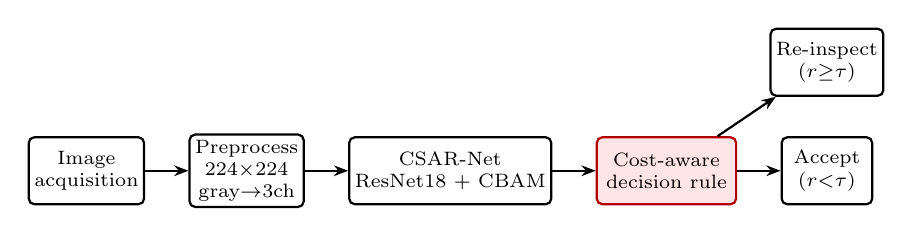
\begin{tikzpicture}[
			box/.style={rectangle,draw,thick,rounded corners=2pt,minimum height=0.85cm,minimum width=1.15cm,font=\scriptsize,align=center,inner sep=2pt},
			key/.style={rectangle,draw=red!70!black,thick,rounded corners=2pt,minimum height=0.85cm,minimum width=1.45cm,font=\scriptsize,align=center,fill=red!10},
			arr/.style={-{Stealth[length=1.8mm]},thick},
		]
			\node[box] (acq) {Image\\acquisition};
			\node[box,right=0.55cm of acq] (pre) {Preprocess\\$224{\times}224$\\gray$\to$3ch};
			\node[box,right=0.55cm of pre] (net) {CSAR-Net\\ResNet18 $+$ CBAM};
			\node[key,right=0.55cm of net] (dec) {Cost-aware\\decision rule};
			\node[box,right=0.55cm of dec] (acc) {Accept\\$(r{<}\tau)$};
			\node[box,above=0.5cm of acc] (re) {Re-inspect\\$(r{\ge}\tau)$};
			\draw[arr] (acq)--(pre);
			\draw[arr] (pre)--(net);
			\draw[arr] (net)--(dec);
			\draw[arr] (dec)--(acc);
			\draw[arr] (dec)--(re);
		\end{tikzpicture}
		\caption{Deployment pipeline of CSAR-Net on a magnetic tile inspection line. Only the classifier training, the evaluation metric, and the decision rule differ from a conventional accuracy-optimized system; the inference-time footprint is identical to the plain ResNet18 backbone.}
		\label{fig:pipeline}
	\end{figure}

	\subsection{Cost--benefit analysis under quality-cost theory}
	\par{
		The recall gains are economically meaningful because miss costs dominate. Under quality-cost theory \citep{juran1993quality}, a miss (a defective tile passed as normal) is an \emph{external failure cost} (the most expensive category), whereas a false alarm is only an internal re-inspection cost. Let $\pi_c$ be the class prior, $\mathrm{FNR}_c=1-\mathrm{Recall}_c$ the miss rate of class $c$, and $\mathrm{FPR}_c$ the rate at which tiles of other classes are falsely routed to re-inspection. The expected cost per inspected tile is
		\begin{equation}
			\mathbb{E}[\mathrm{cost}]=\sum_{c=1}^{K}\pi_c\Bigl[\mathrm{FNR}_c\,C_{\mathrm{miss}}^{(c)}+\mathrm{FPR}_c\,C_{\mathrm{re}}\Bigr],
			\label{eq:cost}
		\end{equation}
		where $C_{\mathrm{miss}}^{(c)}$ is the external-failure cost of missing class $c$ and $C_{\mathrm{re}}$ is the much smaller re-inspection cost of a false alarm. Because safety-critical misses satisfy $C_{\mathrm{miss}}^{(c)}\gg C_{\mathrm{re}}$, the first term dominates, and a method that raises the recall of a costly class while holding false alarms roughly fixed yields an economic gain even when average accuracy is unchanged.
	}

	\par{
		On the test split ($\approx$269 tiles) this is concrete rather than hypothetical. Table \ref{tbl:cost} computes the expected miss and false-alarm counts from the 3-seed recall means and the per-class test counts. The CE baseline misses $\approx$22.3 defect tiles and falsely flags $\approx$3.2 defect-free tiles; CBAM misses $\approx$19.0 defect tiles and falsely flags $\approx$4.4. In other words, CBAM saves about $3.4$ defect misses at the price of about $1.1$ extra false alarms per $\approx$269 tiles; since $C_{\mathrm{miss}}\gg C_{\mathrm{re}}$, the net saving $\approx 3.4\,C_{\mathrm{miss}}-1.1\,C_{\mathrm{re}}$ is strongly positive. In contrast, the LDAM-stacked variant that forces break recall up through aggressive reweighting simultaneously drags defect-free recall down to 0.838 (Fig.~\ref{fig:recallbar}), flooding the re-inspection queue with $\approx$31 false alarms: the over-correction failure expressed in cost terms. The decision threshold can be set by trading the ROC against the enterprise's actual $C_{\mathrm{miss}}/C_{\mathrm{re}}$ ratio \citep{provost1998cost,elkan2001cost}, an instance of cost-sensitive learning applied to the \emph{decision rule} rather than to the feature or loss layer \citep{elkan2001cost,he2009learning}.
	}

	\begin{table}[pos=htbp]
		\footnotesize
		\caption{Expected miss and false-alarm counts per test set ($\approx$269 tiles), computed from the 3-seed recall means and per-class test counts. CBAM saves $\approx$3.4 defect misses at the price of $\approx$1.1 extra false alarms.}
		\label{tbl:cost}
		\centering
		\begin{tabular}{lcc}
			\hline
			\textbf{Quantity (per $\approx$269 tiles)} & \textbf{CE} & \textbf{CBAM} \\ \hline
			Blowhole misses ($n{=}23$) & 5.3 & 3.7 \\
			Break misses ($n{=}17$) & 8.7 & 7.7 \\
			Crack misses ($n{=}11$) & 2.3 & 2.3 \\
			Fray misses ($n{=}6$) & 0.7 & 1.0 \\
			Uneven misses ($n{=}21$) & 5.3 & 4.3 \\
			Total defect misses & 22.3 & 19.0 \\
			Defect-free false alarms ($n{=}191$) & 3.2 & 4.4 \\ \hline
		\end{tabular}
	\end{table}

	\begin{figure}[pos=htbp]
		\centering
		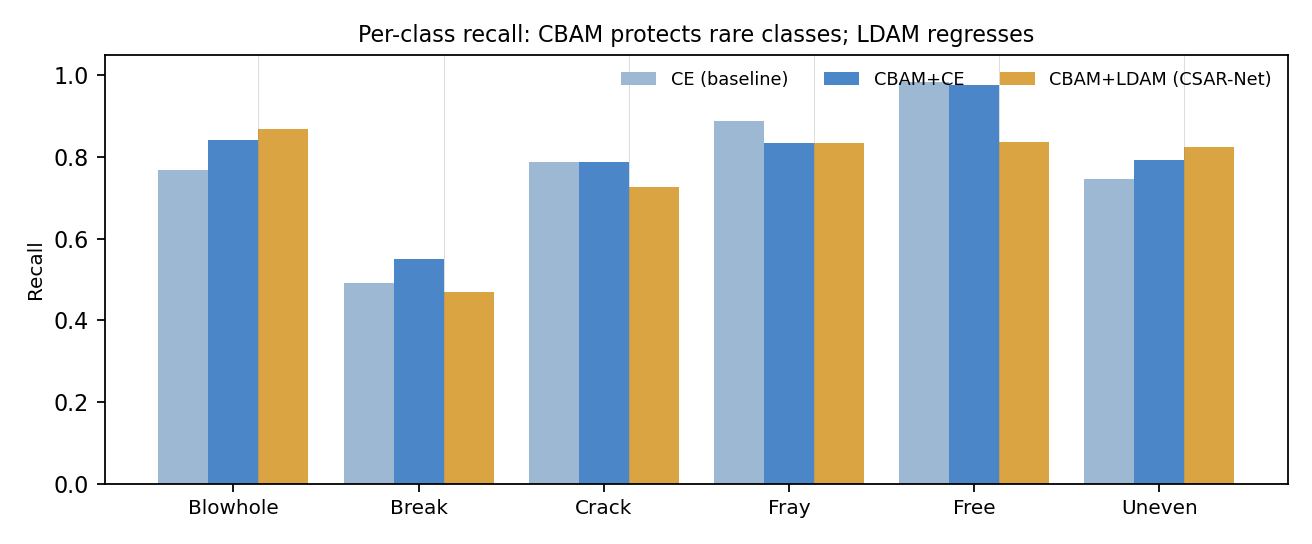
\includegraphics[width=0.92\textwidth]{./figures/fig_recall_bar.png}
		\caption{Per-class recall of CE, CBAM$+$CE, and CBAM$+$LDAM on MTSD (3-seed mean). CBAM lifts the rare, costly classes (break, blowhole, uneven) while keeping defect-free recall nearly intact; stacking LDAM pulls break and defect-free recall back down.}
		\label{fig:recallbar}
	\end{figure}

	\subsection{Design guidance and generalization}
	\par{
		For practitioners building a long-tailed industrial classifier, the ablation (Fig.~\ref{fig:ablbars}) condenses into an actionable recipe: (i) add a label-agnostic channel$+$spatial attention block to the deep residual stages; this is the single robust gain and requires no hyperparameter beyond the standard CBAM; (ii) keep the objective as plain cross-entropy, or a small margin at most, and avoid aggressive class-balanced reweighting, which over-corrects on scarce real defects \citep{he2009learning,drummond2003c4}; (iii) evaluate with macro G-mean, never average accuracy. The recipe transfers across backbones and domains: the same CBAM blocks attach to a larger ResNet or a lightweight MobileNet \citep{howard2017mobilenets,sandler2018mobilenetv2} for different throughput budgets, and the imbalance-aware evaluation is expected to carry over to other long-tailed industrial surfaces: steel (NEU-DET) \citep{song2013noise}, metallic parts \citep{tao2018defect}, and deployment-oriented surface-defect systems \citep{tabernik2020segmentation,roth2022towards}, and industrial anomaly-detection benchmarks \citep{bergmann2019mvtec}. Detection-based pipelines (from YOLO \citep{redmon2016you,bochkovskiy2020yolov4} to segmentation networks \citep{ronneberger2015u}) and alternative backbones (deeper ResNets \citep{he2016deep}, EfficientNet \citep{tan2019efficientnet}, and vision transformers \citep{dosovitskiy2021image,liu2021swin}) share the same long-tailed label structure, so the feature-layer attention rule should transfer. Resampling remedies such as SMOTE \citep{chawla2002smote} remain complementary when a scarce class has enough structure to synthesize, and recent surveys \citep{bhatt2021image} catalog the wider surface-defect landscape. Calibrating the exact cost ratio with enterprise quality-cost data, and few-shot adaptation to novel defect types, are the natural next steps for deployment.
	}

	\begin{figure}[pos=htbp]
		\centering
		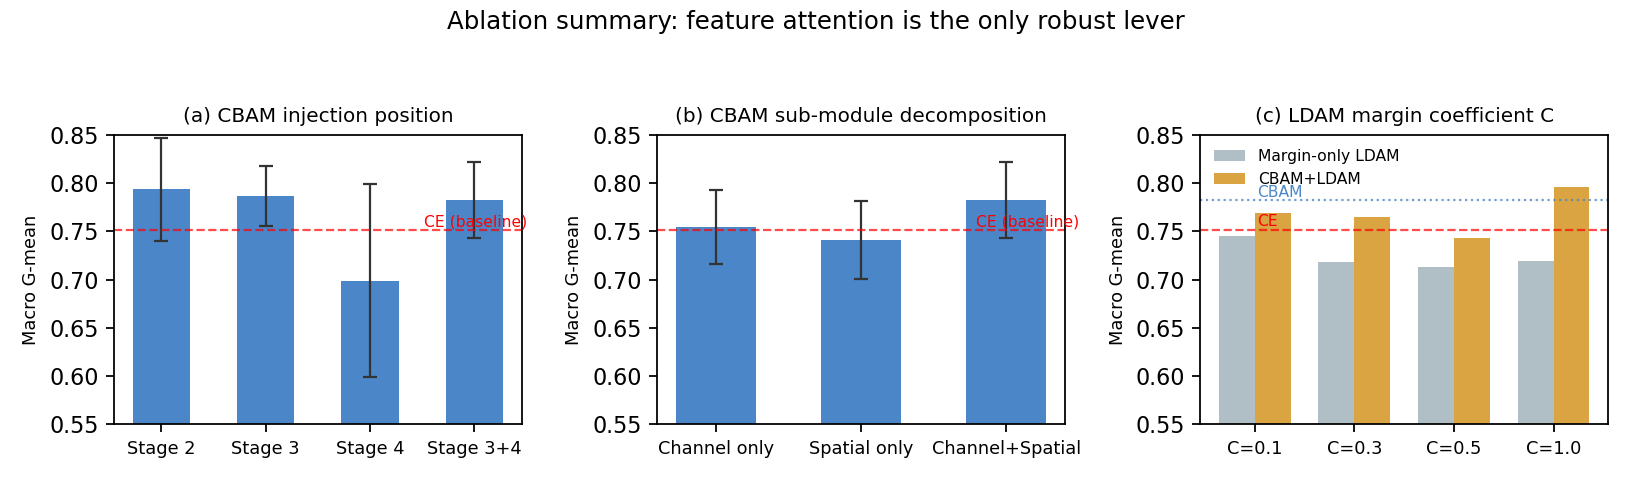
\includegraphics[width=0.95\textwidth]{./figures/fig_ablation_bars.png}
		\caption{Ablation summary: (a) injection position is robust except for stage 4 alone; (b) neither channel-only nor spatial-only clears the baseline; (c) the CBAM$+$LDAM combination is non-monotonic and fragile in the margin coefficient $C$. Feature-layer attention is the only robust lever.}
		\label{fig:ablbars}
	\end{figure}

	\subsection{Limitations, deployment risks, and reproducibility}
	\par{
		A number of caveats bound the transfer of these results to a production line. First, the study is single-dataset: every conclusion is drawn on MTSD, and cross-domain transfer to steel (NEU-DET), metal parts, or PCB is argued by analogy rather than by direct experiment, so the magnitude of the CBAM gain on other surfaces remains to be measured. Second, seed-to-seed variance is non-trivial (macro G-mean standard deviations of $0.03$--$0.05$); the $+3.1$pp CBAM gain is robust relative to this noise, but the finer ordering among the top three injection positions is not. Third, the cost asymmetry is proxied by the inverse class frequency rather than by an enterprise's measured quality-cost ledger, so a deployment should replace this proxy with an actual $C_{\text{miss}}/C_{\text{re}}$ ratio. Fourth, the classifier is closed-world: novel defect types absent from training are necessarily misclassified, so an open-set or anomaly-detection wrapper \citep{bergmann2019mvtec,roth2022towards} is advisable. On the reproducibility side the pipeline is deliberately simple and fully deterministic: it is implemented in PyTorch \citep{paszke2019pytorch}, the ResNet18 backbone is trained from scratch on MTSD (grayscale replicated to three $224\times224$ channels) without ImageNet pretraining, and the model is optimized with Adam \citep{kingma2015adam} (learning rate $10^{-3}$, weight decay $10^{-4}$, cosine annealing, 40 epochs, batch size 32) over three seeds; fixed cuDNN settings remove algorithm nondeterminism, and every ablation reuses the identical recipe. ImageNet pretraining \citep{krizhevsky2012imagenet} and multi-surface validation are the most immediate extensions for even scarcer domains.
	}

	\clearpage
	%% 7. Conclusion
	\section{Conclusion}
	\label{sec:conclusion}
	\par{
		This paper addresses long-tailed, cost-asymmetric magnetic tile surface defect recognition and proposes a Cost-Sensitive Attention Residual Network, CSAR-Net, assembled from three decoupled modules: a ResNet18 backbone for hierarchical feature extraction, CBAM for label-agnostic feature-layer attention, and LDAM for label-dependent loss-layer cost calibration. On MTSD, feature-layer attention is the robust lever: CBAM raises macro G-mean from 0.752 to 0.782 ($+$3.1pp, the lowest variance) and lifts the recall of the hardest, costliest break defect from 0.490 to 0.549. A complete ablation localizes the source of the gain and the cause of the degradation: feature attention is the only stable gain, every form of loss-layer cost calibration over-corrects ($-$3.8pp to $-$8.6pp), stacking LDAM on CBAM dilutes the attention gain to $-$0.8pp, and injecting the cost signal into attention (CS-CBAM) necessarily collapses. These findings translate into a clear design rule for long-tailed inspection systems: align the metric with miss costs via macro G-mean, and protect the rare, costly classes through feature-layer attention rather than through loss-layer reweighting.
	}

	\begin{table}[pos=htbp]
		\footnotesize
		\caption{Summary of findings and their design implications. Each finding maps to a concrete, transferable rule for long-tailed inspection systems.}
		\label{tbl:findings}
		\centering
		\resizebox{\textwidth}{!}{%
		\begin{tabular}{lll}
			\hline
			\textbf{Finding} & \textbf{Evidence} & \textbf{Design implication} \\ \hline
			Feature attention is the robust gain & CBAM $+$3.1pp, lowest variance & Add label-agnostic attention to deep stages \\
			Loss-layer calibration over-corrects & LDAM $-$8.6 / margin $-$3.8 / reweight $-$4.8pp & Keep cross-entropy (or a small margin) \\
			Stacking LDAM on CBAM dilutes the gain & CSAR-Net 0.744 vs.\ CBAM 0.782 & Do not stack calibration onto attention \\
			Injecting cost into attention collapses & CS-CBAM G-mean $\to$0 in all seeds & Keep attention label-agnostic; cost at decision rule \\ \hline
		\end{tabular}}
	\end{table}

	\par{
		The limitations are as follows: the experiments are on a single magnetic tile dataset, and per-class recall varies across the 3 seeds; generalization to other industrial surfaces (steel, PCB, castings) remains to be verified; and the cost asymmetry is currently proxied by class frequency rather than an enterprise's actual quality-cost data. Future work will extend to more industrial defect datasets, explore stronger backbones and minority-class generation, and calibrate precise cost structures with enterprise quality-cost data in real production lines.
	}

	\section*{CRediT authorship contribution statement}
	\par{[First author]: Conceptualization, Methodology, Supervision, Funding acquisition, Writing - Review \& Editing. Chenyang Xie: Methodology, Software, Investigation, Validation, Formal analysis, Writing - Original Draft.}

	\section*{Declaration of competing interest}
	\par{The authors declare that they have no known competing financial interests or personal relationships that could have appeared to influence the work reported in this paper.}

	\section*{Funding}
	\par{This work was jointly supported by the following projects: [to be filled].}

	\section*{Acknowledgements}
	\par{The authors would like to thank the reviewers for their insightful comments and useful suggestions.}

	\section*{Data and code availability}
	\par{The source code, training configuration, and figure-generation scripts that reproduce the experiments reported in this paper are openly available at \url{https://github.com/otreeevol/csar_net}. The Magnetic Tile Surface Defects (MTSD) dataset is a public benchmark introduced by \citet{huang2020surface} and was used as released; no new data were generated in this study. Trained model checkpoints are not distributed in the public repository because of their size, and are available from the corresponding author on reasonable request.}

	%% Bibliography
	\bibliographystyle{model5-names}
	\bibliography{csar_refs}

\end{sloppypar}
\end{document}
